\part{ÉTUDE ET RÉALISATION}

\chapter{Cadrage, analyse et conception}

\textit{Comme tout problème qui a été clairement défini, il faut le réaliser mais nous ne pouvons
	parler d’implémentation sans toutefois faire une analyse et une conception. Pour ce faire,
	nous allons cadrer le projet en utilisant la méthode CPS, suivi d’une analyse
	fonctionnelle et non fonctionnelle et bien sûr terminer par une conception des architectures
	physique et logique.}

\clearpage

\section{Cadrage du projet}

\subsection{Le projet}

\subsubsection{Le nom}

Le projet à réaliser consiste à pouvoir dispenser les cours (médecine, mathématiques, chimie)
du système éducatif et le travail portera sur le module d’apprentissage de la chimie, d’où le
nom \textbf{vredu chemistry lab}.

\subsubsection{Définition succincte}

\textbf{vredu chemistry lab} sera développée pour la plateforme de réalité virtuelle et les navigateurs web. Elle se devra donc d’être compatible non seulement avec tous les casques de réalité virtuelle de la marque OCULUS mais aussi avec tous les appareils disposant d’un navigateur web. Il sera ainsi possible pour un enseignant de programmer une expérience chimique sur un navigateur web afin que l'apprenant puisse la suivre sur son casque de réalité virtuelle.

\subsubsection{Caractéristiques essentielles}

Notre application sera caractérisée par :

\begin{itemize}
	\item Une accessibilité sur tous les formats d’équipements numériques de la marque oculus et sur les appareils disposant d’un navigateur web,
	\item Prise en charge des éléments permettant d’effectuer une réaction chimique (éléments du tableau périodique, éprouvettes, béchers, centrifugeuses…).
\end{itemize}

\subsubsection{Motifs qui sous-tendent ce projet}

De nos jours, l’univers numérique offre énormément d'opportunités en ce qui concerne l'acquisition de connaissance grâce à la grande quantité d’informations échangées. 
La chimie est une science dont l'apprentissage se fait de façon expérimentale, expériences entourées de contraintes auxquelles une solution digitale pourrait être la solution à savoir :

\begin{itemize}
	\item Annuler la contrainte du lieu des expériences.
	\item Annuler la contrainte liée à l’acquisition et à la maintenance du matériel d'expérimentation.
	\item Limiter des risques d’accidents durant les expérimentations.
	\item Diminuer les couts de maintenance et d’acquisition du matériel de laboratoire.
\end{itemize}

\subsection{Les objectifs}

\subsubsection{Objectifs techniques}
\begin{itemize}
	\item \textbf{\underline{Résultats attendus}} : A la fin de ce projet, nous devons avoir deux applications, une pour le web permettant à un enseignant de chimie la création de réactions chimiques auxquelles les apprenants participent par le billet de la seconde application qui elle tournera dans un environnement immersif virtuel.
	\item \textbf{\underline{Objectif principal}} : Obtenir un laboratoire de chimie virtuelle permettant la simulation des réactions chimiques.
	\item \textbf{\underline{Objectifs secondaires}} :
	      \begin{itemize}
		      \item Représenter les réactifs et les produits en trois dimensions et de façon réaliste et immersive
		      \item Calculer la quantité de matière des réactifs dans une solution
		      \item Calculer la concentration des réactifs dans une solution
		      \item Calculer la masse molaire moléculaire des réactifs dans une solution
		      \item Calculer le ph d’une solution
	      \end{itemize}
\end{itemize}

\subsubsection{Objectifs de délai}

L’application doit être réalisée dans un délai de sept mois à compter de la date du 10 mai 2022.

\subsubsection{Objectifs de coûts}

\paragraph{Estimation de la main d’œuvre}


\begin{enumerate}
	\item \textbf{Les différents modèles d'estimation des coûts et ressources d’un projet}

	      Au cours de nos recherches, nous avons trouvé de nombreux modèles d’estimation des coûts et ressources d’un projet. Nous pouvons entre autres parlé de :

	      \begin{enumerate}
		      \item \textbf{La méthode descendante} : reste extrêmement populaire dans la gestion de projets contemporains. L'expression « top-down » (descendante) signifie que les instructions sont données en amont. Les objectifs du projet sont fixés par la direction.
		      \item \textbf{La méthode ascendante} : elle se caractérise par une participation proactive de l'équipe dans le processus d'exécution du projet. Les membres de l'équipe sont invités à participer à toutes les étapes du processus de gestion. L'ensemble de l'équipe est amené à décider de la marche à suivre.
		      \item \textbf{La méthode COCOMO} : (acronyme de l'anglais Constructive Cost Model) est un modèle permettant de définir une estimation de l'effort à fournir dans un développement logiciel et la durée que ce dernier aura en fonction des ressources allouées.
	      \end{enumerate}

	      Sachant que la majeure partie du travail est consacrée à la production du logiciel, nous nous inspirons de la méthode COCOMO pour estimer les coûts de la ressource humaine à ce niveau, lesquels coûts seront inclus dans les coûts globaux de la solution envisagée.

	\item \textbf{Le modèles d'estimation des coûts COCOMO}

	      Cocomo (Constructive Cost Model) est un modèle de régression basé sur le LOC, c’est-à-dire le nombre de lignes de code. Il s’agit d’un modèle procédural d’estimation des coûts pour les projets logiciels et souvent utilisé comme processus de prédiction fiable des divers paramètres associés à la réalisation d’un projet, tels que la taille, l’effort, le coût, le temps et la qualité. Il a été proposé par Barry Boehm en 1970 et repose sur l’étude de 63 projets, ce qui en fait l’un des modèles les mieux documentés. Différents modèles de Cocomo ont été proposés pour prédire l’estimation des coûts à différents niveaux, en fonction de la précision et de l’exactitude requises. Tous ces modèles peuvent être appliqués à une variété de projets, dont les caractéristiques déterminent la valeur de constante à utiliser dans les calculs ultérieurs. Ces caractéristiques propres à différents types de systèmes sont mentionnées ci-dessous :

	      \begin{enumerate}
		      \item \textbf{Organique} – Un projet logiciel est dit de type organique si la taille de l’équipe requise est suffisamment petite, si le problème est bien compris et a été résolu dans le passé et si les membres de l’équipe ont une expérience nominale du problème.
		      \item \textbf{Semi-détaché} – Un projet logiciel est dit de type semi-détaché si les caractéristiques vitales telles que la taille de l’équipe, l’expérience, la connaissance des différents environnements de programmation se situent entre celles de l’organique et de l’Embedded. Les projets classés comme semi-détachés sont comparativement moins familiers et difficiles à développer par rapport aux projets organiques et nécessitent plus d’expérience et une meilleure orientation et créativité. Ex : Les compilateurs ou différents Systèmes Embarqués peuvent être considérés de type Semi-Détachés.
		      \item \textbf{Intégré} – Un projet logiciel nécessitant le plus haut niveau de complexité, de créativité et d’expérience entre dans cette catégorie. Un tel logiciel nécessite une taille d’équipes plus importantes que les deux autres modèles et les développeurs doivent également être suffisamment expérimentés et créatives pour développer des modèles aussi complexes.
	      \end{enumerate}

	      \begin{table}[h!]
		      \caption {types de projet COCOMO}
		      \begin{tabularx}{\textwidth} {
				      | >{\raggedright\arraybackslash}X
				      | >{\centering\arraybackslash}X
				      | >{\raggedleft\arraybackslash}X |}
			      \hline
			      \textbf{Type de projet} & \textbf{Effort en Homme Mois} & \textbf{Temps de Développement} \\
			      \hline
			      ORGANIQUIE              & $2.4(KDSI)^{1.05}$            & $2.5(HM)^{0.38}$                \\
			      \hline
			      MEDIAN                  & $3.0(KDSI)^{1.12}$            & $2.5(HM)^{0.35}$                \\
			      \hline
			      IMBRIQUÉ                & $3.6(KDSI)^{1.20}$            & $2.5(HM)^{0.32}$                \\
			      \hline
		      \end{tabularx}
	      \end{table}

	      Le projet est estimé à 20 KDSI (nombre de milliers d’instructions source livrées) en mode organique (Il est défini par une innovation minimale, une organisation simple en petites équipes expérimentées).

	      % \widowpenalties 3 10000
	      % \raggedbottom
	      \textbf{Formule} :
	      \[E\footnote{E = Effort en Personne-Mois}=2.4\cdot{KLOCx}^{1.05}\]
	      \[D\footnote{D = Durée en Mois.}=2.5\cdot E^{0.38}\]

	      \textbf{Application numérique} :

	      \[E=2.4\cdot10^{1.05}\approx27 Personnes/Mois\]
	      \[D=2.5\cdot 56^{0.38}\approx8 Mois\]

	      \begin{table}[h!]
		      \caption {Estimation des coûts}
		      \begin{tabularx}{\textwidth} {
				      | >{\raggedright\arraybackslash}X
				      | >{\centering\arraybackslash}X
				      | >{\centering\arraybackslash}X
				      | >{\centering\arraybackslash}X
				      | >{\raggedleft\arraybackslash}X |}
			      \hline
			      \textbf{Participant}                    & \textbf{Quantité} & \textbf{Durée en semaine} & \textbf{Cout/Semaine} & \textbf{Cout total} \\
			      \hline
			      \textbf{Chef de projet / concepteur}                 & 1                 & 4                         & 200.000 XAF           & 800.000 XAF         \\
			      \hline
			      \textbf{Développeur}                    & 1                 & 32                        & 100.000 XAF           & 3.200.000 XAF       \\
			      \hline
			      \textbf{Testeur}                        & 2                 & 1                         & 50.000 XAF            & 50.000 XAF          \\
			      \hline
			      \multicolumn{4}{| l |}{\textbf{Total} } & 4.050.000 XAF                                                                               \\
			      \hline
		      \end{tabularx}
	      \end{table}
\end{enumerate}

\paragraph{Estimation matérielle et logiciel}\mbox{}\\

Ce tableau présente une estimation du matériel selon le besoin et la durée.

\begin{table}[H]
	\caption{Estimation des coûts matériels}

	\begin{tabular}{ |p{7cm}|p{2cm}|p{3cm}|p{3cm}| }
		\hline
		\textbf{Ressource}                                                                                                                                                                                                                                     & \textbf{Nombre de payement} & \textbf{Cout par payement}                   & \textbf{Total} \\
		\hline
		Desktop monté avec les caractéristiques : 32Go de RAM, Une carte graphique Nvidia GeForce GTX 1070, 250Go de disque dur SSD, 1To de disque dur HDD, Processeur Intel core i7 3.60GHz, Boitier et carte graphique predator, Ecran 32 pouces, Clavier HP & 7                           & 23.472 XAF (\textit{Amortissement par mois}) & 164.304 XAF    \\
		\hline
		1 serveur de développement : 100 Go SSD, 4 Go Ram, Ubuntu 20                                                                                                                                                                                           & 7                           & 80.000 XAF                                   & 560.000 XAF    \\
		\hline
		1 serveur git: 2Go RAM, 30 Go HDD, Ubuntu 20                                                                                                                                                                                                           & 7                           & 80.000 XAF                                   & 560.000 XAF    \\
		\hline
		1 casque oculus                                                                                                                                                                                                                                        & 7                           & 5.940 XAF (\textit{Amortissement par mois})  & 41.580 XAF     \\
		\hline
		Connexion Internet haut débit                                                                                                                                                                                                                          & 7                           & 30.000 XAF                                   & 210.000 XAF    \\
		\hline
		Rider                                                                                                                                                                                                                                                  & 1                           & 91.809 XAF                                   & 91.809 XAF     \\
		\hline
		Unreal engine                                                                                                                                                                                                                                          & 7                           & Gratuit                                      & Gratuit        \\
		\hline
		Webstorm                                                                                                                                                                                                                                               & 1                           & 91.809 XAF                                   & 91.809 XAF     \\
		\hline
		\multicolumn{3}{| l |}{\textbf{Total} }                                                                                                                                                                                                                & 1.719.502 XAF                                                                               \\
		\hline
	\end{tabular}
\end{table}

Le coût du matériel est ainsi estimé à : \textbf{1.719.502 XAF}

Ainsi le coût total du projet est de \textbf{5.769.502 XAF }

\subsection{La technique}

\subsubsection{La base sur laquelle le projet s’appuie}

Nous avons déjà eu à réaliser des projets en informatique et en particulier des applications Web, bien que les applications de réalités virtuelles soient pour nous une nouvelle expérience, nous pensons pouvoir y parvenir grâce la communauté qui est nombreuse et également l’aide des professionnels en stage notamment notre encadreur. De plus, les supports de cours, les enseignants et l’internet (possibilité de documentation) sont des atouts majeurs renforçant cet engagement. Des didacticiels dans des environnement 3D existent déjà, ce qui nous fait croire encore plus à la réalisation de ce projet.

\subsubsection{Les difficultés principales de ce projet}

\begin{itemize}
	\item Apporter du réalisme aux réactions chimiques
	\item Sécurité de l’application
\end{itemize}

\subsubsection{Les solutions de repli en cas de problème }

Pour le problème lié au réalisme à apporter aux expériences, nous avons pensé à confier la réalisation des assets 3D à des tiers que nous paierons.

En ce qui concerne la sécurité de l’application, vu que l’application sera hébergée en ligne nous nous informerons sur les différents risques liés à un tel hébergement et tenterons de les éviter lors de la phase de développement.

\subsection{Le planning}

\subsubsection{Dates clés}

\begin{itemize}
	\item Date de début : 10 mai 2022
	\item Date de fin :  03 décembre 2022
\end{itemize}

\subsubsection{Grandes phases du planning}

Pour la gestion du temps, il existe des méthodes de planification prévisionnelle de projet tel que le diagramme de Gantt. Ce dit diagramme regroupe toutes les tâches, les durées et les ressources ordonnées de manière graduelle permettant à toute l’équipe de suivre son évolution. Il peut être modifié au fur et à mesure en fonction des délais respectés ou pas ainsi que des imprévus. Dans le cadre de notre projet, la planification de nos tâches nous a permis de ressortir le diagramme de Gantt suivant :


\begin{table}[H]
	\caption{Estimation des coûts matériels}
	\resizebox{\textwidth}{!}{%
		\begin{tabular}{|lll|l|ll|}
			\hline
			\multicolumn{1}{|l|}{\textbf{Phase}}                            & \multicolumn{2}{l|}{\textbf{Taches}}                                    & \textbf{\begin{tabular}[c]{@{}l@{}}Durée\\  en jour\end{tabular}}                  & \multicolumn{1}{l|}{\textbf{Durée en heure}} & \textbf{Prédécesseurs}         \\ \hline
			\multicolumn{1}{|l|}{\multirow{4}{*}{\textbf{Analyse}}}         & \multicolumn{2}{l|}{Cadrage du projet (A)}                              & 4                                                    & \multicolumn{1}{l|}{36}                      &                                \\ \cline{2-6}
			\multicolumn{1}{|l|}{}                                          & \multicolumn{2}{l|}{Etude l’existant (B)}                               & 5                                                    & \multicolumn{1}{l|}{45}                      & A                              \\ \cline{2-6}
			\multicolumn{1}{|l|}{}                                          & \multicolumn{2}{l|}{Elaboration du diagramme des cas d’utilisation (C)} & 3                                                    & \multicolumn{1}{l|}{27}                      & B                              \\ \cline{2-6}
			\multicolumn{1}{|l|}{}                                          & \multicolumn{2}{l|}{Elaboration des diagrammes de séquence (D)}         & 3                                                    & \multicolumn{1}{l|}{27}                      & B                              \\ \hline
			\multicolumn{1}{|l|}{\multirow{2}{*}{\textbf{Conception}}}      & \multicolumn{2}{l|}{Elaboration du diagramme de classe (E)}             & 5                                                    & \multicolumn{1}{l|}{45}                      & D,C                            \\ \cline{2-6}
			\multicolumn{1}{|l|}{}                                          & \multicolumn{2}{l|}{Elaboration du diagramme de déploiement (F)}        & 1                                                    & \multicolumn{1}{l|}{9}                       & D,C                            \\ \hline
			\multicolumn{1}{|l|}{\multirow{11}{*}{\textbf{Implémentation}}} & \multicolumn{1}{l|}{\multirow{4}{*}{Back end}}                          & Module de gestion des utilisateurs (G)               & 15                                           & \multicolumn{1}{l|}{135} & F   \\ \cline{3-6}
			\multicolumn{1}{|l|}{}                                          & \multicolumn{1}{l|}{}                                                   & Module de gestion des éléments chimiques (H)         & 12                                           & \multicolumn{1}{l|}{108} & G,E \\ \cline{3-6}
			\multicolumn{1}{|l|}{}                                          & \multicolumn{1}{l|}{}                                                   & Module de gestion des équipements de laboratoire (I) & 15                                           & \multicolumn{1}{l|}{135} & H   \\ \cline{3-6}
			\multicolumn{1}{|l|}{}                                          & \multicolumn{1}{l|}{}                                                   & Tests (J)                                            & 2                                            & \multicolumn{1}{l|}{18}  & I   \\ \cline{2-6}
			\multicolumn{1}{|l|}{}                                          & \multicolumn{1}{l|}{\multirow{4}{*}{Front end}}                         & Module de gestion des utilisateurs (K)               & 15                                           & \multicolumn{1}{l|}{135} & J   \\ \cline{3-6}
			\multicolumn{1}{|l|}{}                                          & \multicolumn{1}{l|}{}                                                   & Module de gestion des éléments chimiques (L)         & 15                                           & \multicolumn{1}{l|}{135} & K   \\ \cline{3-6}
			\multicolumn{1}{|l|}{}                                          & \multicolumn{1}{l|}{}                                                   & Module de gestion des équipements de laboratoire (M) & 10                                           & \multicolumn{1}{l|}{90}  & L   \\ \cline{3-6}
			\multicolumn{1}{|l|}{}                                          & \multicolumn{1}{l|}{}                                                   & Tests (N)                                            & 2                                            & \multicolumn{1}{l|}{18}  & M   \\ \cline{2-6}
			\multicolumn{1}{|l|}{}                                          & \multicolumn{1}{l|}{\multirow{3}{*}{Interfaces 3D}}                     & Menus et interface d’accueil (O)                     & 10                                           & \multicolumn{1}{l|}{90}  & N   \\ \cline{3-6}
			\multicolumn{1}{|l|}{}                                          & \multicolumn{1}{l|}{}                                                   & Gestion des réactions chimiques (P)                  & 25                                           & \multicolumn{1}{l|}{225} & N   \\ \cline{3-6}
			\multicolumn{1}{|l|}{}                                          & \multicolumn{1}{l|}{}                                                   & Tests (Q)                                            & 5                                            & \multicolumn{1}{l|}{45}  & O,P \\ \hline
			\multicolumn{1}{|l|}{\textbf{Transition}}                       & \multicolumn{2}{l|}{Tests (R)}                                          & 5                                                    & \multicolumn{1}{l|}{45}                      & Q                              \\ \hline
			\multicolumn{3}{|l|}{\textbf{Total}}                            & \textbf{152}                                                            & \multicolumn{2}{l|}{\textbf{1368}}                                                                                                   \\ \hline
		\end{tabular}%
	}
\end{table}

Ce tableau nous permettra de réaliser notre diagramme Gantt.

\subsubsection{Diagramme Gantt}

Ce diagramme présente le planning général du projet, fait en utilisant le logiciel Gantt Project.

\begin{figure}[H]
	\centering
	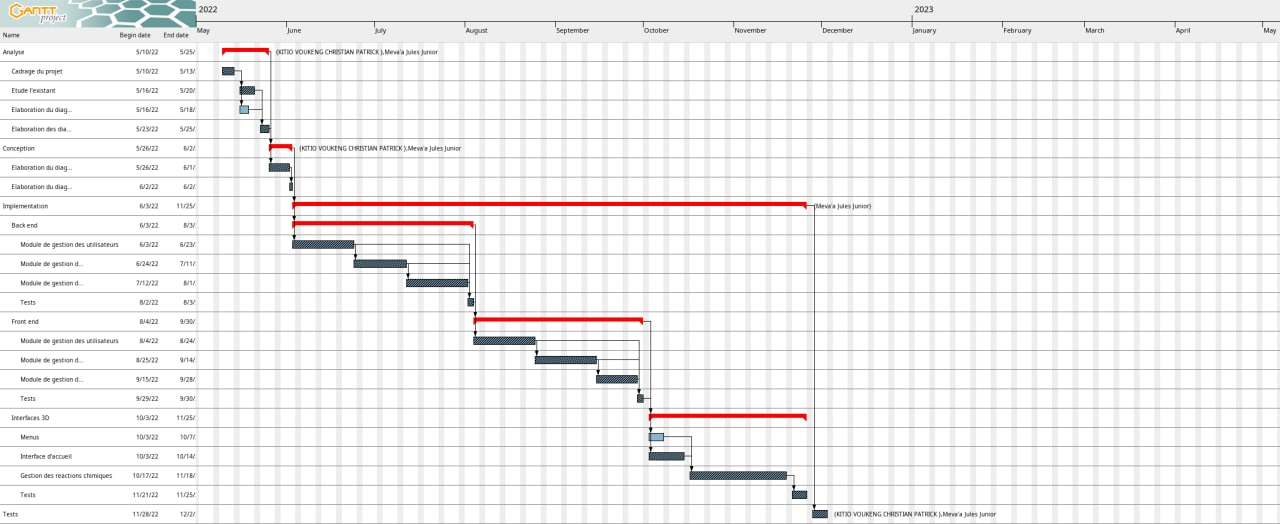
\includegraphics[width=1.3\textwidth, angle=-90]{img/gantt}
	\caption{Diagramme de gantt du projet}
	\label{fig:mesh1}
\end{figure}

De ce diagramme, ressort la date de début du projet qui est le 10 mai 2022 et la date de fin le 03 Décembre 2022. La durée du projet est de 156 jours. Le chemin critique est noté en bleu sombre sur ce diagramme.

\subsection{Les moyens}

\subsubsection{Moyens humains}

Ici nous retrouvons l'équipe chargée de la réalisation du module \textbf{M. KITIO VOUKENG Christian PATRICK} directeur technique a monglo-technologie et \textbf{MEVA’A JULES JUNIOR} stagiaire en développement et en management des solutions digitales et datas a monglo-technologie.

\subsubsection{Moyens matériels}

\begin{table}[H]
	\centering
	\caption{Moyens matériels}
	\label{tab:my-table}
	\begin{tabular}{|l|p{7cm}|}
		\hline
		\multicolumn{1}{|l|}{Ordinateurs desktop} & 32Go de RAM, Une carte graphique Nvidia GeForce GTX 1070, 250Go de disque dur SSD, 1To de disque dur HDD, Processeur Intel core i7 3.60GHz, Boitier et carte graphique predator, Ecran 32 pouces, Clavier HP \\ \hline
		\multicolumn{2}{|l|}{\begin{tabular}[c]{@{}l@{}}1 Casque de réalité virtuelle Oculus \\ Quest\end{tabular}}                                                                                                                                                                                                         \\ \hline
		\multicolumn{2}{|l|}{1 serveur git}                                                                                                                                                                                                                      \\ \hline
		\multicolumn{2}{|l|}{1 serveur git}                                                                                                                                                                                                                      \\ \hline
	\end{tabular}
\end{table}

\subsection{Le management du projet}

Pour la réalisation de ce projet, nous disposons des ressources humaines suivantes :

\begin{table}[H]
	\centering
	\caption{Le management du projet}
	\label{tab:my-table}
	\resizebox{\textwidth}{!}{%
		\begin{tabular}{|l|l|}
			\hline
			\textbf{Noms}                       & \textbf{Fonctions}                         \\ \hline
			M. KITIO VOUKENG CHRISTIAN PATRICK & Responsable du projet, analyste et testeur \\ \hline
			MEVA’A JULES JUNIOR                 & Analyste, développeur et testeur           \\ \hline
		\end{tabular}%
	}
\end{table}

\subsection{La communication}


\subsubsection{Communication interne du projet}

\begin{itemize}
	\item Collaboration via GitLab
	\item Communication via telegram
	\item Réunion en présentielle ou en ligne (en fonction du contexte) pour l’évaluation de l’évolution du projet et les tests
\end{itemize}

\subsubsection{Communication externe}

\begin{itemize}
	\item Avec les encadreurs académiques
	      \begin{itemize}
		      \item La communication avec l’encadreur se fera par des séances de travail en présentielles et parfois par moyens téléphoniques.
	      \end{itemize}
	\item Avec les potentiels client
	      \begin{itemize}
		      \item Information des corps administratif, professoral et estudiantin via les réseaux sociaux (twitter, groupes WhatsApp, Facebook, telegram) de l’existence de l’application.
		      \item Publication des affiches et spots publicitaires
		      \item Descente dans les établissements
	      \end{itemize}
\end{itemize}

\section{Analyse du système}

\subsection{Analyse fonctionnelle} % (fold)
\label{sub:analyse-fonctionnelle}

Il s’agit là des fonctionnalités que doivent posséder le système :

\subsubsection{Idedntification des acteurs} % (fold)
\label{ssub:Idedntification-des-acteurs}

% subsubsection Idedntification des acteurs (end)

Un acteur représente un rôle joué par une entité externe (utilisateur humain, dispositif matériel ou autre système) qui interagit directement avec le système étudié. Un acteur peut consulter et/ou modifier directement l’état du système, en émettant et/ou en recevant des messages susceptibles d’être porteurs de données. Dans le cas de notre application, nous avons pu identifier ces différents acteurs :

\begin{itemize}
	\item L’administrateur : il est chargé de la modération de l'application en ayant accès à toutes les fonctionnalités de la version web de l'application.
	\item L’enseignant : c'est celui qui crèe les réactions chimiques dans le système.
	\item L’apprenant : c'est celui qui effectue les réations dans un casque de réalité virtuelle.
\end{itemize}

\subsubsection{Identification des cas d’utilisation}

Il est question ici de ressortir une manière d’utiliser le système et d’en décrire les exigences fonctionnelles. Nous avons retenu les cas d’utilisation suivants :

% Please add the following required packages to your document preamble:
% \usepackage{multirow}
\begin{table}[H]
	\centering
	\caption{Les acteurs du systeme et leurs cas d'utilisation}
	\label{tab:my-table}
	\begin{tabular}{|l|p{10cm}|}
		\hline
		\textbf{Acteurs}                         & \textbf{Cas d’utilisations}                                                           \\ \hline
		\textbf{L’apprenant}                     & Effectuer une réaction chimique                                                       \\ \hline
		\multirow{6}{*}{\textbf{L’enseignant}}   & S’inscrire                                                                            \\ \cline{2-2}
		                                         & Se connecter                                                                          \\ \cline{2-2}
		                                         & Consulter son compte                                                                  \\ \cline{2-2}
		                                         & Modifier son compte                                                                   \\ \cline{2-2}
		                                         & Supprimer son compte                                                                  \\ \cline{2-2}
		                                         & Créer, Lister, Modifier, activer, désactiver et supprimer des éléments chimiques      \\ \hline
		\multirow{5}{*}{\textbf{Administrateur}} & Effectuer tous les cas d’utilisation de l’enseignant                                  \\ \cline{2-2}
		                                         & Lister, activer, désactiver, modifier et supprimer un compte utilisateur.             \\ \cline{2-2}
		                                         & Lister, activer, désactiver, modifier et supprimer toutes les réactions chimiques.    \\ \cline{2-2}
		                                         & Lister, activer, désactiver, modifier et supprimer tous les éléments chimiques        \\ \cline{2-2}
		                                         & Créer, lister, modifier, activer, désactiver et supprimer du matériel de laboratoire. \\ \hline
	\end{tabular}
\end{table}

\subsubsection{Diagramme des cas d’utilisation}

Les diagrammes de cas d'utilisation sont des diagrammes utilisés pour une représentation du comportement fonctionnel d'un système logiciel. Ils permettent d’avoir une vue d’ensemble entre les fonctionnalités d’un système et les acteurs qui en bénéficient.

\begin{figure}[H]
	\centering
	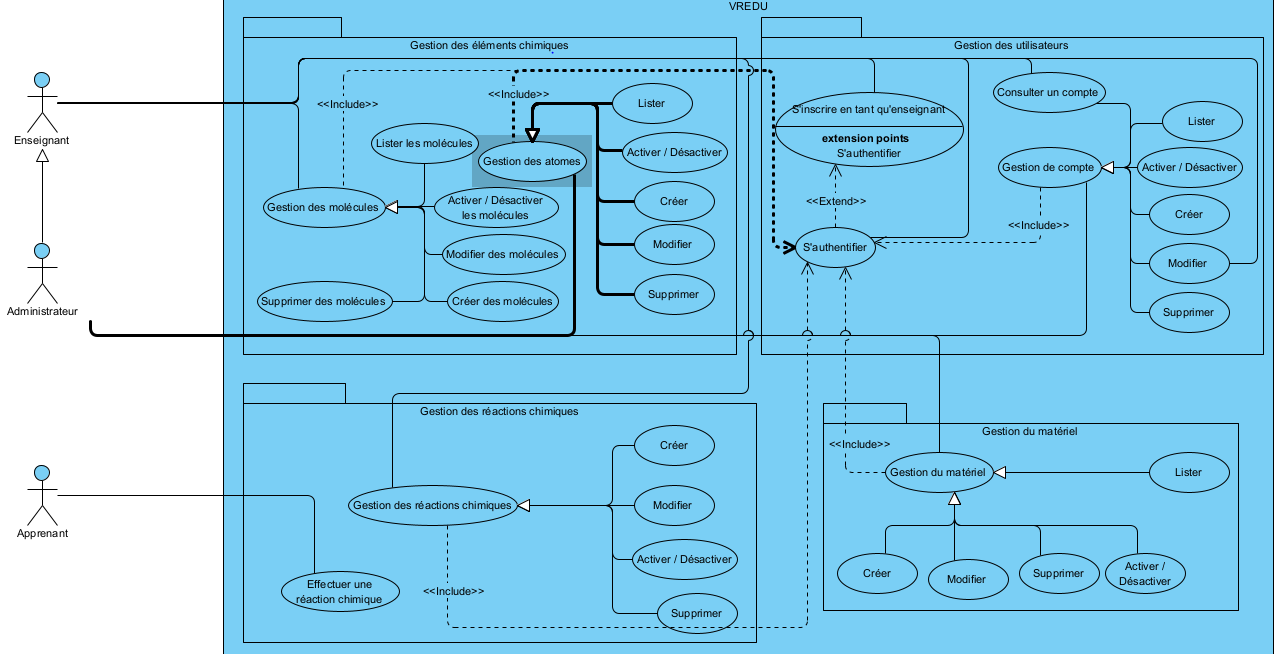
\includegraphics[trim={10cm 0 0 0}, width=1\textwidth]{img/ucd}
	\caption{Diagramme des cas d’utilisation}
	\label{fig:mesh1}
\end{figure}

De ce diagramme ressortent les différents groupe fonctionnalités du module de chimie de l’application VREDU à savoir :  le module de gestion des utilisateurs qui permettra la gestion des compte utilisateur (administrateur et enseignant), le module de gestion des éléments chimique qui permettra les opérations de création, modification. Activation et désactivation des éléments chimiques, le module de gestion des réactions chimiques et le module de gestion du matériel de laboratoire.

\subsubsection{Description textuelle de quelques cas d’utilisation}

\begin{itemize}
	\item \textbf{S’authentifier}
	      \begin{itemize}
		      \item Sommaire d’identification
		            \begin{itemize}
			            \item Titre : s’authentifier
			            \item Acteurs : Administrateur et enseignant
			            \item Objectif : Il permet à l’acteur de s’identifier et se connecter en saisissant son login et mot de passe.
		            \end{itemize}
		      \item Description des scénarios
		            \begin{itemize}
			            \item Précondition : L’acteur doit avoir ouvert l’application
			            \item Post condition :
			                  \begin{itemize}
				                  \item Acteur connecté.
				                  \item Ouverture de l’interface utilisateur.
			                  \end{itemize}
			            \item Scénario nominal
			                  \begin{enumerate}
				                  \item L’acteur demande à ouvrir la page de connexion
				                  \item Le système affiche la page de connexion
				                  \item L’acteur saisit le nom d’utilisateur et son mot de passe
				                  \item Le système vérifie les données
				                  \item Le système connecte l’acteur et affiche l’interface utilisateur
			                  \end{enumerate}
			            \item Scénario alternatif
			                  \begin{itemize}
				                  \item A. Erreur de connexion : nom d'utilisateur ou mot de passe non valide

				                        Cet enchaînement démarre au point 4

				                  \item 5. Le système affiche un message d’erreur correspondant au problème d’identifiants incorrectes.
				                  \item B. Erreur de connexion : le compte est désactivé

				                        Cet enchaînement démarre au point 4

				                  \item 5. Le système affiche un message d’erreur correspondant au problème de compte désactive
			                  \end{itemize}
		            \end{itemize}
	      \end{itemize}
	\item \textbf{Création d’élément chimique }
	      \begin{itemize}
		      \item Sommaire d’identification
		            \begin{itemize}
			            \item Titre : Création d’élément chimique
			            \item Acteurs : Administrateur et enseignant
			            \item Objectif : Il permet à l’acteur de créer un élément chimique pour la plateforme.
		            \end{itemize}
		      \item Description des scénarios
		            \begin{itemize}
			            \item Précondition : Acteur connecté.
			            \item Post condition :
			                  \begin{itemize}
				                  \item Elément chimique crée dans la base de données.
			                  \end{itemize}
			            \item Scénario nominal
			                  \begin{enumerate}
				                  \item L’acteur demande du formulaire de création des éléments
				                  \item Le système affiche le formulaire de création des éléments
				                  \item L’acteur soumet le formulaire de création
				                  \item Le système vérifie les données
				                  \item Le système enregistre l’élément chimique et réinitialise le formulaire
			                  \end{enumerate}
			            \item Scénario alternatif
			                  \begin{itemize}
				                  \item A. Erreur information soumise incorrects

				                        Cet enchaînement démarre au point 4

				                  \item 5. Le système affiche un message d’erreur pour informations soumises incorrect.
			                  \end{itemize}
		            \end{itemize}
	      \end{itemize}

	\item \textbf{Effectuer une réaction}
	      \begin{itemize}
		      \item Sommaire d’identification
		            \begin{itemize}
			            \item Titre : Effectuer une réaction
			            \item Acteurs : Apprenant
			            \item Objectif : Il permet à l’acteur de réaliser une réaction chimique sur la plateforme.
		            \end{itemize}
		      \item Description des scénarios
		            \begin{itemize}
			            \item Précondition : Application ouverte.
			            \item Post condition :
			                  \begin{itemize}
				                  \item L'interface de réalisation des réactions ouverte.
			                  \end{itemize}
			            \item Scénario nominal
			                  \begin{enumerate}
				                  \item L’acteur demande le formulaire d'identification des réactions
				                  \item Le système affiche le formulaire d'identification des réactions
				                  \item L’acteur saisi l'identifiant d'une réaction et soumet le formulaire
				                  \item Le système recherche a réaction
				                  \item Le système envoie de l'interface de réalisation de la réaction
				                  \item L’acteur effectue un mélange et l’envoie
			                  \end{enumerate}
			            \item Scénario alternatif
			                  \begin{itemize}
				                  \item A. Erreur réaction introuvable.

				                        Cet enchaînement démarre au point 4

				                  \item 5.  Le système affiche un message d’erreur pour réaction introuvable.
				                  \item B. Erreur réaction désactivée
				                  \item 5. Le système affiche un message d’erreur pour réaction désactivée
			                  \end{itemize}
		            \end{itemize}
	      \end{itemize}

	\item \textbf{Création d’une réaction}
	      \begin{itemize}
		      \item Sommaire d’identification
		            \begin{itemize}
			            \item Titre : Création d’une réaction
			            \item Acteurs : Administrateur et enseignant
			            \item Objectif : Il permet à l’acteur de créer une réaction chimique pour la plateforme.
		            \end{itemize}
		      \item Description des scénarios
		            \begin{itemize}
			            \item Précondition : Acteur connecté.
			            \item Post condition :
			                  \begin{itemize}
				                  \item Réaction chimique crée dans la base de données.
			                  \end{itemize}
			            \item Scénario nominal
			                  \begin{enumerate}
				                  \item L’acteur demande à créer une réaction
				                  \item Le système retourne le formulaire de création
				                  \item L’acteur envoie les informations sur la réaction
				                  \item Le système demande une confirmation de création.
				                  \item L’acteur confirme la création
				                  \item Le système enregistre la réaction
			                  \end{enumerate}
			            \item Scénario alternatif
			                  \begin{itemize}
				                  \item A. L’acteur annule la création

				                        Cet enchaînement démarre au point 4

				                  \item 5. Le système annule la création.

				                        Le scénario reprend au point 3
			                  \end{itemize}
		            \end{itemize}
	      \end{itemize}

	\item \textbf{Suppression d’une réaction }
	      \begin{itemize}
		      \item Sommaire d’identification
		            \begin{itemize}
			            \item Titre : Suppression d’une réaction
			            \item Acteurs : Administrateur et enseignant
			            \item Objectif : Il permet à l’acteur de supprimer une réaction sur la plateforme.
		            \end{itemize}
		      \item Description des scénarios
		            \begin{itemize}
			            \item Précondition : Acteur connecté.
			            \item Post condition :
			                  \begin{itemize}
				                  \item La réaction est supprimée de la base de données de l’application.
			                  \end{itemize}
			            \item Scénario nominal
			                  \begin{enumerate}
				                  \item L’acteur demande de la liste des réactions
				                  \item Le système retourne la liste des réactions
				                  \item L’acteur sélectionne une réaction
				                  \item Le système demande une confirmation de suppression.
				                  \item L’acteur confirme la suppression
				                  \item Le système supprime la réaction
			                  \end{enumerate}
			            \item Scénario alternatif
			                  \begin{itemize}
				                  \item A. L’acteur annule la suppression

				                        Cet enchaînement démarre au point 4

				                  \item 5. Le système annule la suppression.

				                        Le scénario reprend au point 3
			                  \end{itemize}
		            \end{itemize}
	      \end{itemize}
\end{itemize}

\newpage
\subsubsection{Diagrammes de séquences}

Les diagrammes de séquences sont la représentation graphique des interactions entre les acteurs et le système selon un ordre chronologique.

\begin{itemize}
	\item \textbf{S’authentifier}

	      \begin{figure}[H]
		      \centering
		      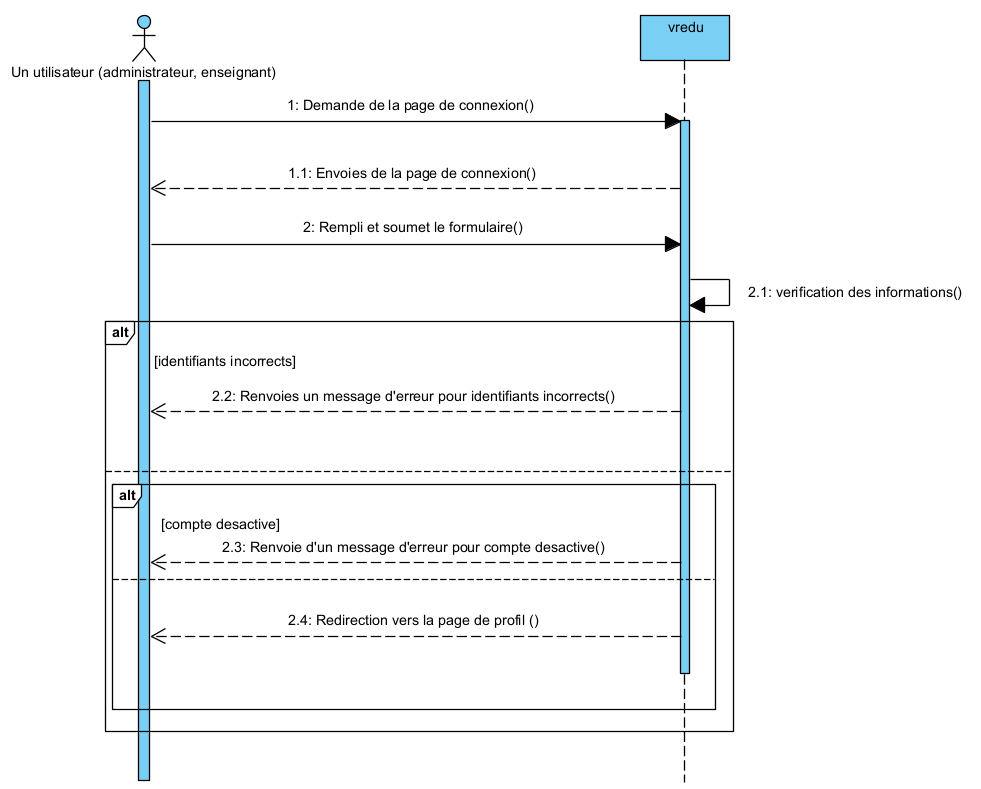
\includegraphics[width=1\textwidth]{img/ucdAuth}
		      \caption{Diagramme de séquence du cas d'utilisation s’authentifier}
		      \label{fig:mesh1}
	      \end{figure}

	      Ce diagramme fait une description détaille du cas d’utilisation d’authentification qui permet à un utilisateur d’être reconnue par le système afin de lui accorder certain droit sur le système en fonction de son identité.

	\newpage
	\item \textbf{Création d’élément chimique}

	      \begin{figure}[H]
		      \centering
		      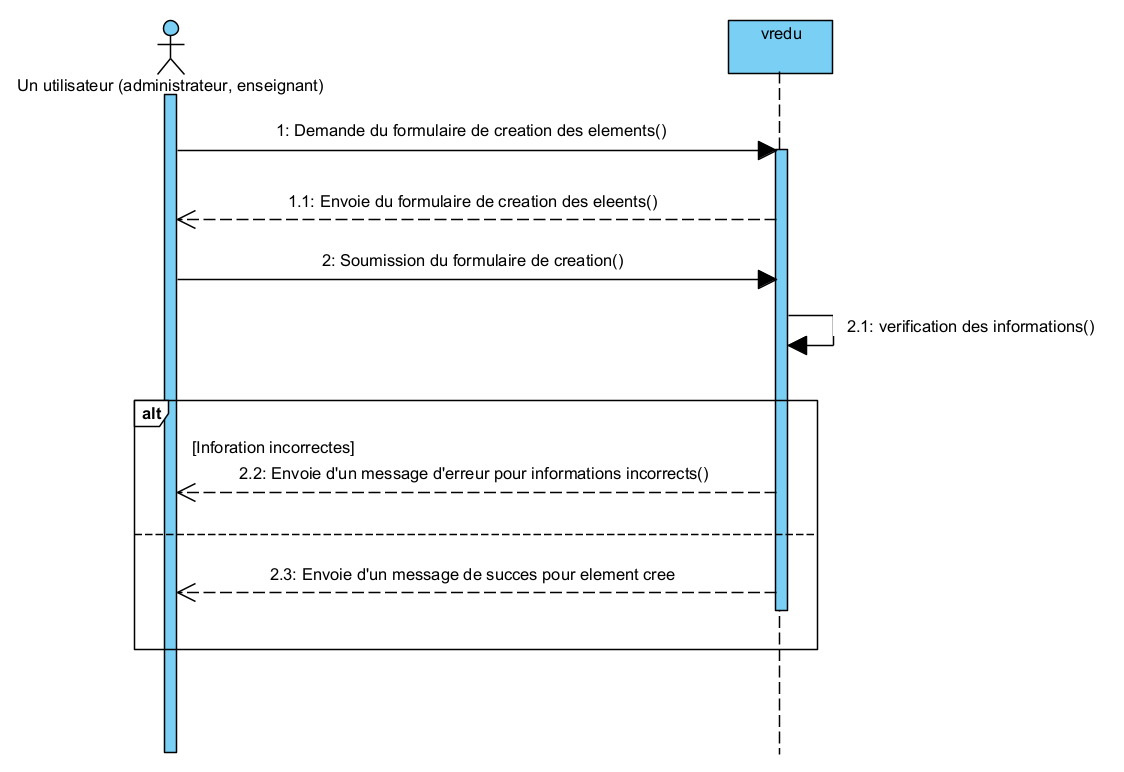
\includegraphics[width=1\textwidth]{img/ucdElCr}
		      \caption{Diagramme de séquence du cas d'utilisation création d’élément chimique}
		      \label{fig:mesh1}
	      \end{figure}

	      Ce diagramme fait une description détaille du cas d’utilisation création d’un élément chimique, ce cas permet à un utilisateur connecte de créer un élément chimique pour une réaction chimique.

	\newpage
	\item \textbf{Effectuer une réaction}

	      \begin{figure}[H]
		      \centering
		      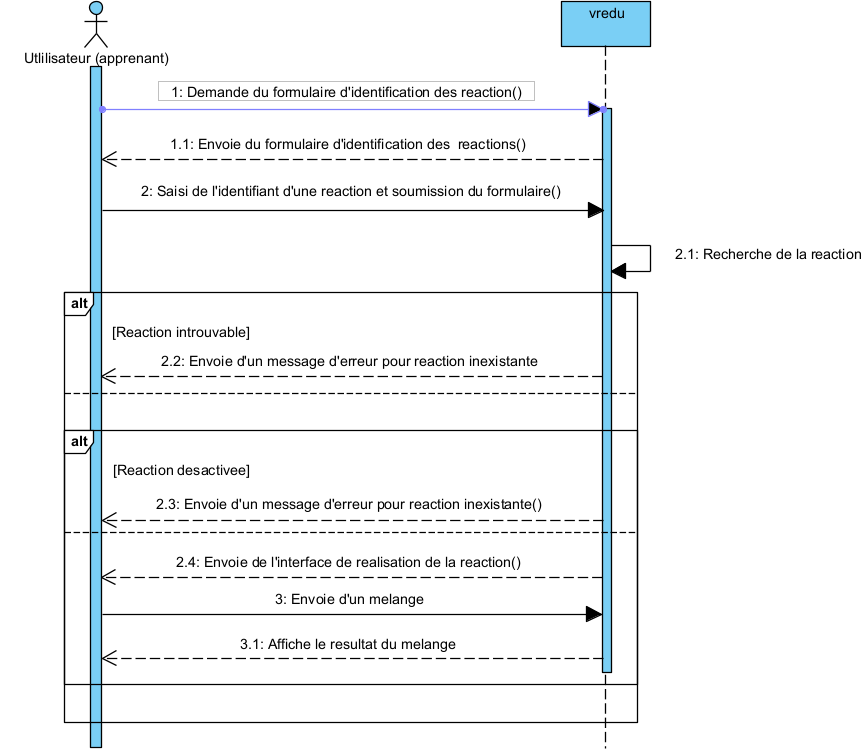
\includegraphics[width=1\textwidth]{img/ucdeur}
		      \caption{Diagramme de séquence du cas d'utilisation effectuer une réaction}
		      \label{fig:mesh1}
	      \end{figure}

	      Ce diagramme fait une description détaille du cas effectuer une réaction qui présente le processus de réalisation d’une réaction chimique sur le système par un apprenant.
\end{itemize}

\newpage
\subsubsection{Diagrammes d’activités}

Les diagrammes d'activités permettent de mettre l'accent sur les traitements. Ils sont donc particulièrement adaptés à la modélisation du cheminement de flots de contrôle et de flots de données. Ils permettent ainsi de représenter graphiquement le comportement d'une méthode ou le déroulement d'un cas d'utilisation.

\begin{itemize}
	\item \textbf{Créer une réaction }

	      \begin{figure}[H]
		      \centering
		      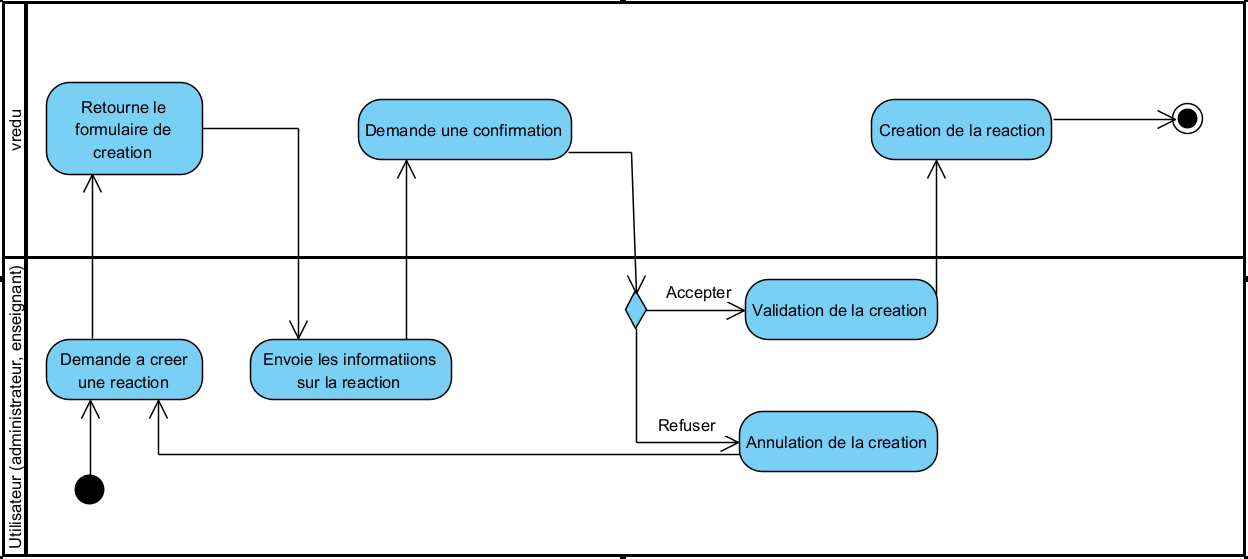
\includegraphics[width=1\textwidth]{img/sdCUR}
		      \caption{Diagramme d’activité du cas d'utilisation créer une réaction}
		      \label{fig:mesh1}
	      \end{figure}

	      Ce diagramme fait une description détaille du cas créer une réaction qui présente le processus de création d’une réaction chimique sur le système par un administrateur ou un enseignant.
	
	\newpage
	\item \textbf{Suppression d’une réaction}

	      \begin{figure}[H]
		      \centering
		      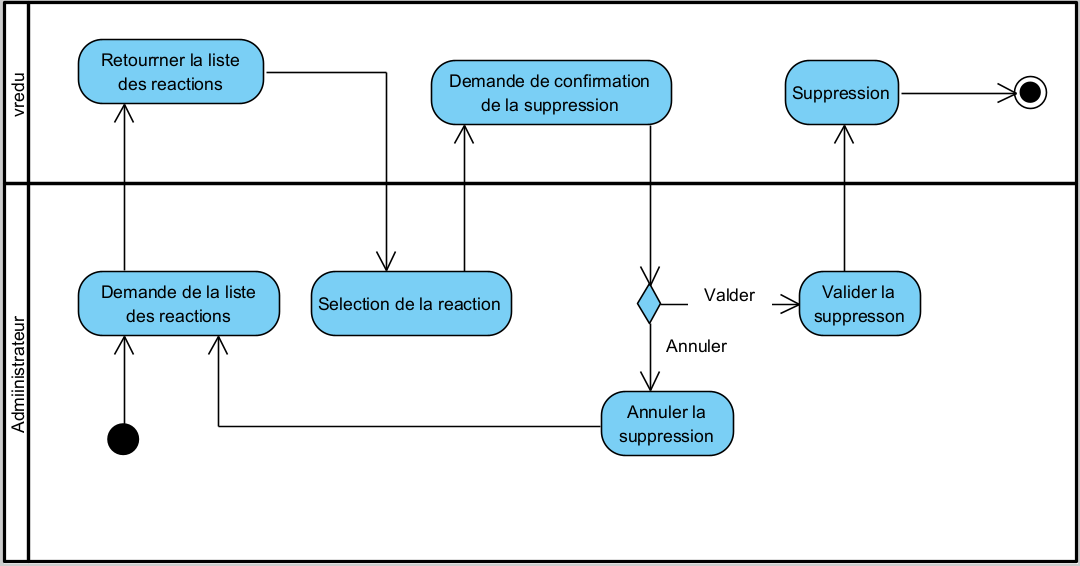
\includegraphics[width=1\textwidth]{img/adsr}
		      \caption{Diagramme d’activité du cas d'utilisation suppression d’une réaction}
		      \label{fig:mesh1}
	      \end{figure}

	      Ce diagramme fait une description détaille du cas suppression d’une réaction qui présente le processus de suppression d’une réaction chimique sur le système par un administrateur ou un enseignant.
\end{itemize}

\newpage
\subsubsection{Diagramme d’état transition}

Un diagramme d'états-transitions est un type de diagramme comportemental en langage de modélisation unifié (UML) qui représente les transitions entre divers objets.

\begin{itemize}
	\item \textbf{Changement d’état des produits d’une réaction}

	      \begin{figure}[H]
		      \centering
		      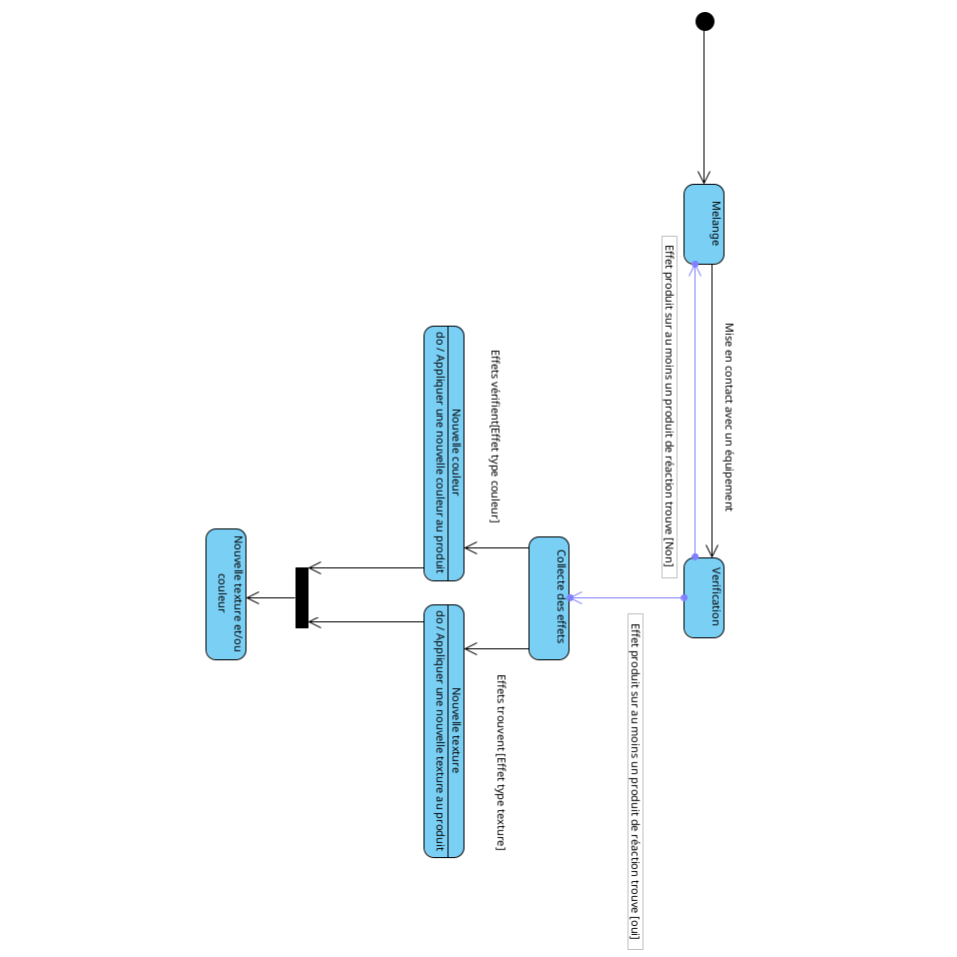
\includegraphics[width=1\textwidth]{img/etdR}
		      \caption{Diagramme d’état transition du cas d'utilisation changement d’état des produits d’une réaction}
		      \label{fig:mesh1}
	      \end{figure}

	      Ce diagramme présente de façon détaillée le processus de changement d’état d’un produit de réaction lors d’une réaction chimique.
	\newpage
	\item \textbf{Changement d’état d'authentification d’un utilisateur }

	      \begin{figure}[H]
		      \centering
		      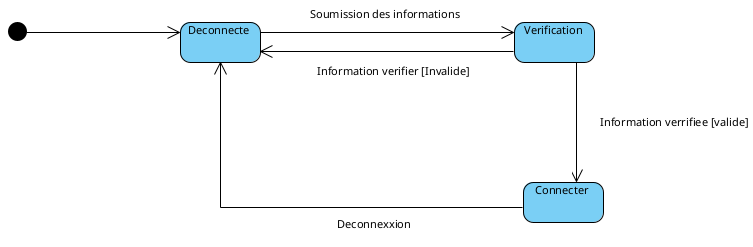
\includegraphics[width=1\textwidth]{img/etu}
		      \caption{Diagramme d’état transition du cas d'utilisation changement d’état d'authentification d’un utilisateur}
		      \label{fig:mesh1}
	      \end{figure}

	      Ce diagramme présente de façon détaillée le changement d’état d’authentification d’un utilisateur en fonction d’évènement effectues sur la plateforme.
\end{itemize}

\subsection{Analyse non fonctionnelle} % (fold)

C’est l’ensemble des exigences qui ne concernent pas spécifiquement le comportement du système mais plutôt identifient des contraintes internes et externes du système. Ainsi les principaux besoins non fonctionnels de notre système sont :

\begin{itemize}
	\item Le code doit être clair, bien structuré pour permettre des futures évolutions du système ;
	\item L’ergonomie : la plateforme doit offrir des interfaces conviviales et faciles à utiliser ;
	\item La sécurité, le système doit garantir un grand niveau de protection des informations sur les utilisateurs.
\end{itemize}

\subsection{Technique et Méthodes} % (fold)

\subsubsection{Choix des techniques de développement}

Plusieurs techniques peuvent être utilisées pour réaliser d’une plateforme web et 3D :

\begin{itemize}
	\item \textbf{Le code pur} :

	      C’est ainsi que les informaticiens créent leur première application. 
		  Il est nécessaire d’avoir de bonnes connaissances en programmation. 
		  En effet toute l'application est créée à partir de ligne de code complètement illisible pour un profane. 
		  Cette solution est longue, couteuse et rarement assez complète pour permettre une modification facile de l’application. 
		  Aujourd’hui, la plupart des développeurs ne créent plus leur application de A à Z, ils utilisent des cadres de travail prédéfinis.

	\item \textbf{Les CMS (Content management system) pour le web} :

	      Ce sont des aides à la création d’applications. Ils ne font pas tous à votre place, mais vous aident en grande partie. Il est très recommandé d’avoir des connaissances en informatique pour réaliser une application à partir d’un CMS. Certains sont en effet très compliqués à mettre en place. De plus aucun hébergement n’est fourni avec le CMS. Il faudra donc mettre en place un serveur HTTP pour héberger son application. Pour finir, la personnalisation du design d’une application sur un CMS est assez fastidieuse. Il sera presque à tous les cas obligatoires de mettre la main dans le code source de   l’application. D’autres techniques existent notamment les Outils en ligne.

	\item \textbf{Framework et librairies} :

	      Il existe également des Framework et librairies (bout de code écrit permettant de faciliter le travail du développeur), qui est l’une des méthodes les plus utilisée dans le monde du développement, nous avons donc optes pour cette méthode et nous allons choisir un Framework parmi ceux existant.
\end{itemize}

\subsubsection{Choix du Framework}

\textbf{ASP.net} pour le \textbf{backend}, \textbf{React} pour le \textbf{frontend} et \textbf{unreal engine} pour la \textbf{3D}. Comme \textbf{SGBD}, nous avons allons utiliser \textbf{PostgreSQL} (le SGBD utilisé par l’entreprise).

\section{Conception du système}

\subsection{Diagramme de classe} % (fold)

Le diagramme de classes est un schéma utilisé pour présenter les classes et les interfaces des systèmes ainsi que leurs relations.

\begin{figure}[H]
	\centering
	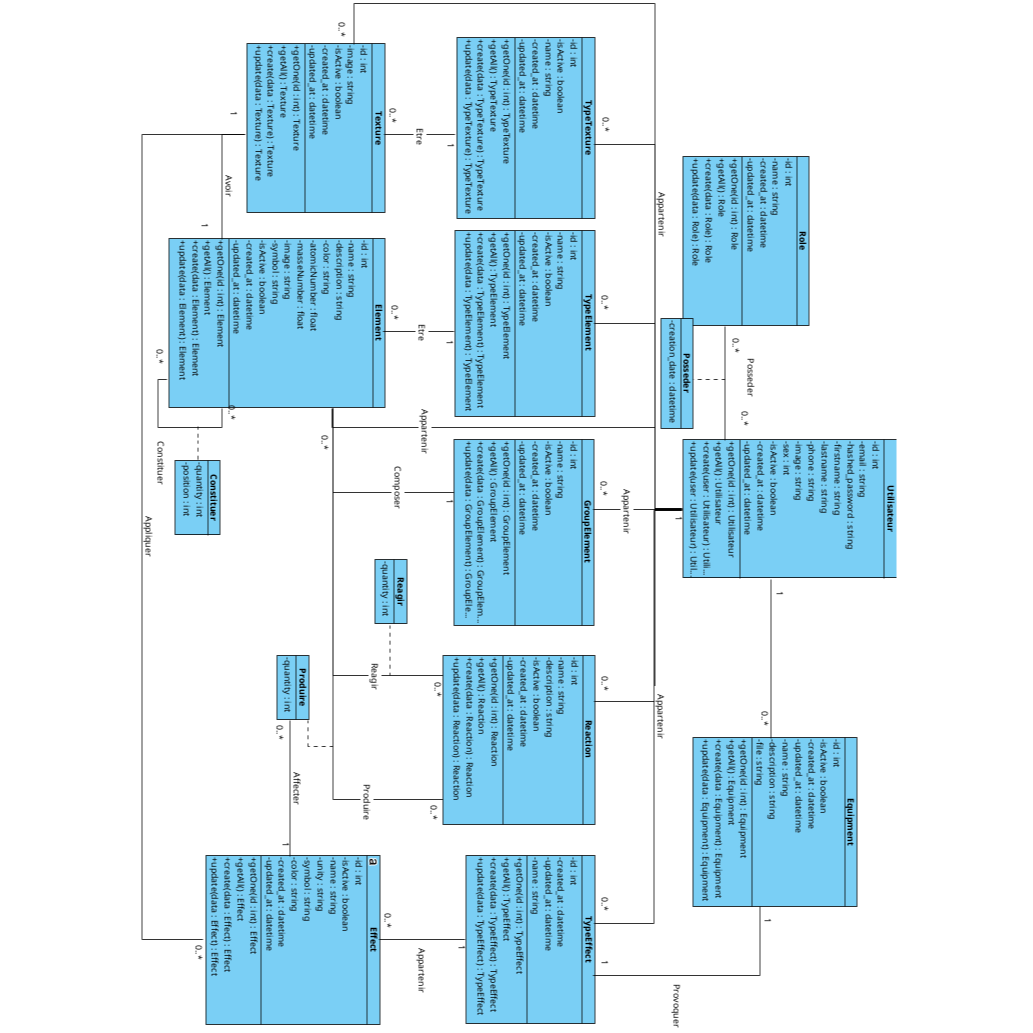
\includegraphics[trim={5cm 0 0 0}, width=1\textwidth]{img/dc}
	\caption{Diagramme de classe du système}
	\label{fig:mesh1}
\end{figure}

Ce diagramme présente les classes et leurs interactions dans le système.

\subsection{Diagramme de déploiement} % (fold)

En UML, un diagramme de déploiement est une vue statique qui sert à représenter l’utilisation de l’infrastructure physique par le système et la manière dont les composants du système sont répartis ainsi que leurs relations entre eux. Les éléments utilisés par un diagramme de déploiement sont principalement les nœuds, les composants, les associations et les artefacts. Les caractéristiques des ressources matérielles physiques et des supports de communication peuvent être précisées par stéréotype.

\begin{figure}[H]
	\centering
	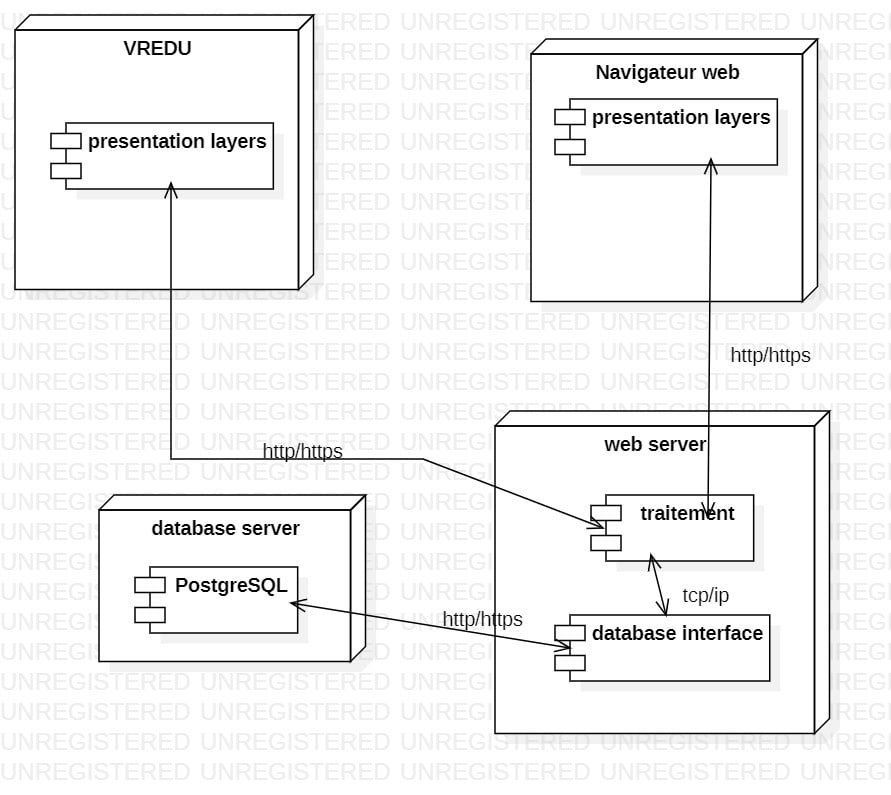
\includegraphics[width=1\textwidth]{img/dd}
	\caption{Diagramme de déploiement du système}
	\label{fig:mesh1}
\end{figure}

\subsection{Quelques maquettes d'IHM (Interface Homme Machine)}

\subsubsection{Page d'accueil}

Cette page de décrire la solution aux enseignants qui souhaites la découvrir.

\begin{figure}[H]
	\centering
	
\includegraphics[width=0.5\textwidth]{img/home}
	\caption{IHM de la page d'accueil}
	\label{fig:mesh1}
\end{figure}

Il y apparait clairement une entête de page avec le logo et les différents liens d'inscription et de connexion.
Les sections suivantes décrivent la solutions, présentent ses statistiques et les contacts en cas de questions ou de problèmes.

\subsubsection{Page d'inscription des enseignants}

Cette page permet la création de compte enseignant en y renseignant les informations personnelles de l'utilisateur.

\begin{figure}[H]
	\centering
	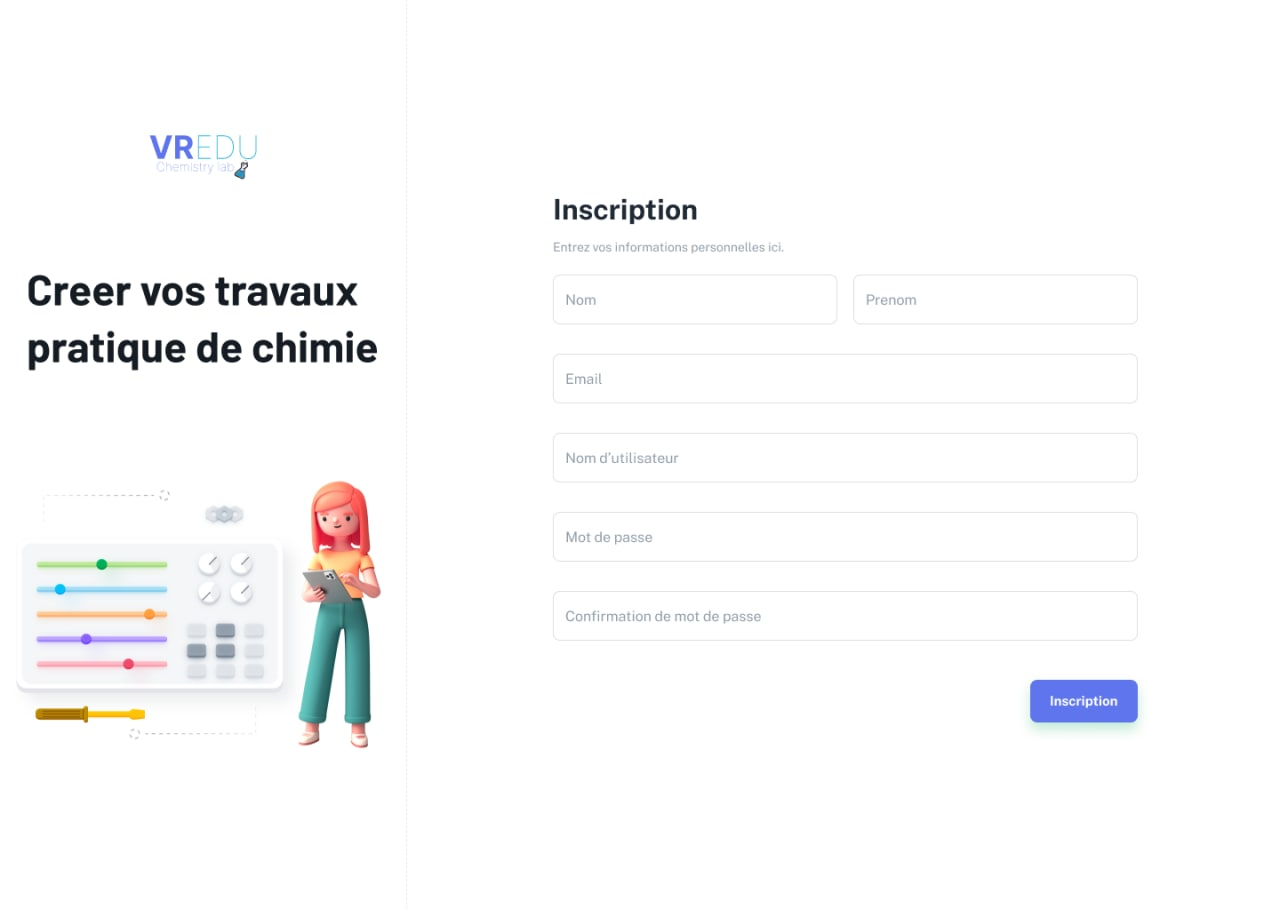
\includegraphics[width=1\textwidth]{img/insc}
	\caption{IHM de la page d'inscription des enseignants}
	\label{fig:mesh1}
\end{figure}

Il y apparait le formulaire de création de compte avec les différents champs remplir avant la soumission.

\subsubsection{Page de connexion des enseignants}

Cette page permet à tous les utilisateurs d’accéder à l’application en utilisant un login et
un mot de passe.

\begin{figure}[H]
	\centering
	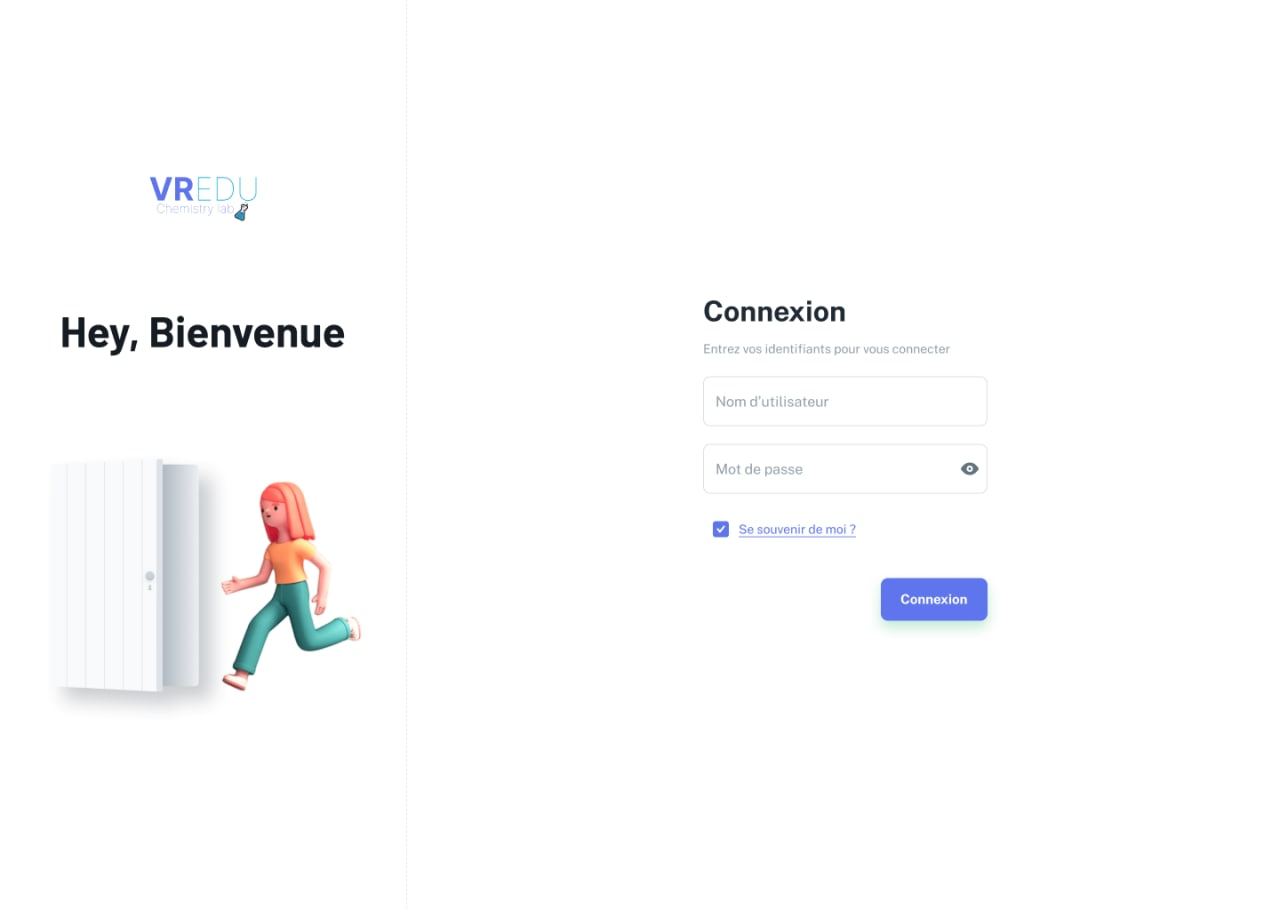
\includegraphics[width=1\textwidth]{img/conn}
	\caption{IHM de la page de connexion des enseignants}
	\label{fig:mesh1}
\end{figure}

Il y apparait le formulaire de connexion avec les champs pour le nom d'utilisateur et le mot de passe à remplir avant soumission.
Deux catégorie d'utilisateurs peuvent utiliser cette interface à savoir les administrateurs et les enseignants.

\subsubsection{Page espace personnel des enseignants et administrateurs}

Cette page permet à l'utilisateur d'avoir un appercu de ses réactions.

\begin{figure}[H]
	\centering
	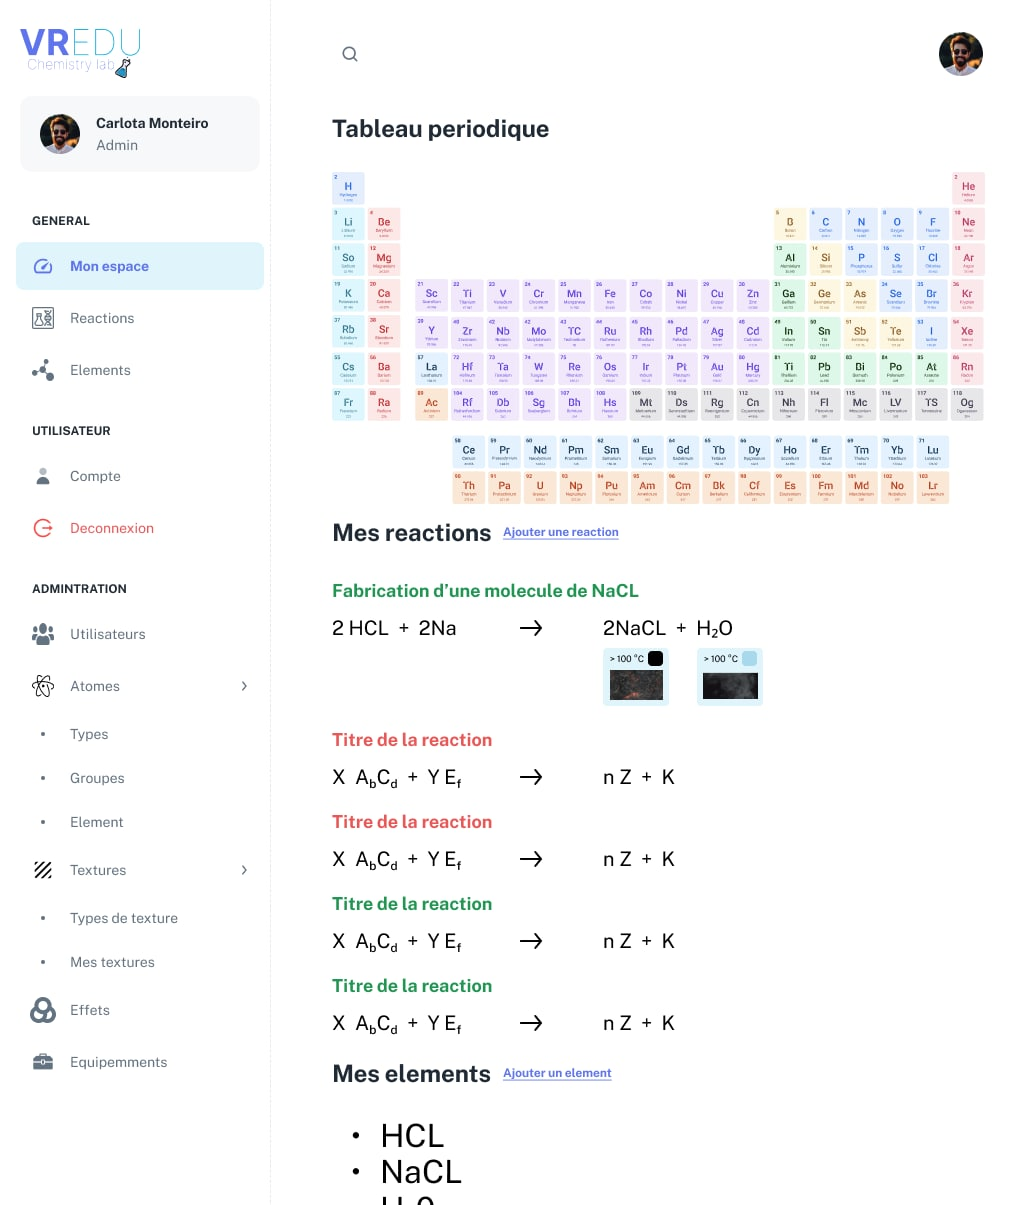
\includegraphics[width=1\textwidth]{img/esp}
	\caption{IHM de la page espace personnel des enseignants et administrateurs}
	\label{fig:mesh1}
\end{figure}

Il y apparait la liste des éléments chimiques du tableau périodique et la liste des réactions de l'utilisateur connecté.

\subsubsection{Interface du laboratoire en vue de dessus}

Cette interface représente une vue de dessus du laboratoire virtuelle ou les apprenant effectuerons leur réactions.

\begin{figure}[H]
	\centering
	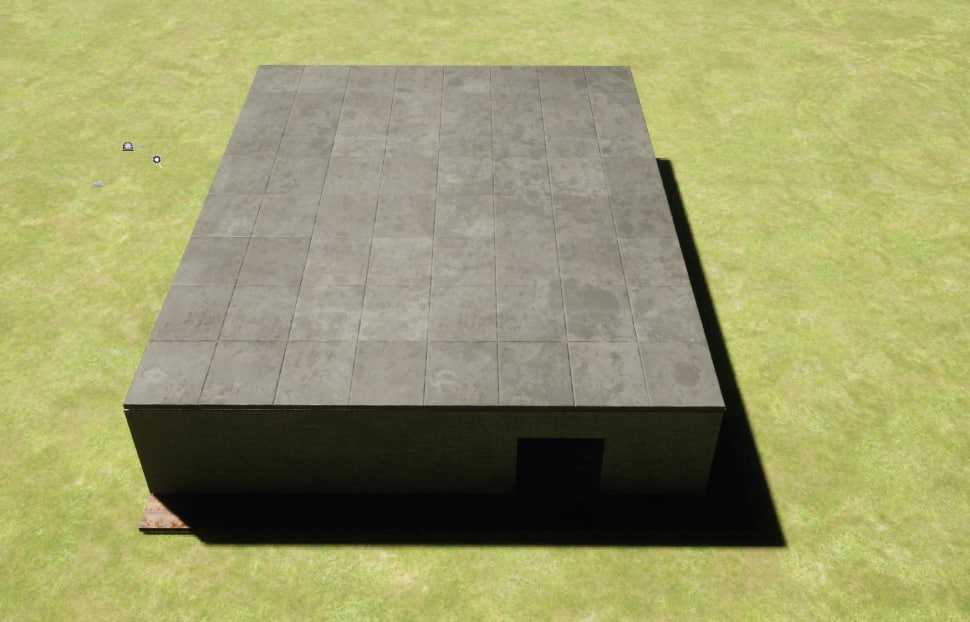
\includegraphics[width=1\textwidth]{img/labot}
	\caption{IHM du laboratoire en vue de dessus}
	\label{fig:mesh1}
\end{figure}

Il y apparait un locale vue du dessus et présente l'environnement extérieur du laboratoire oû aurons lieu les réactions.

\subsubsection{Interface du laboratoire en vue de face}

Cette interface représente une vue de face du laboratoire virtuelle ou les apprenant effectuerons leur réactions.

\begin{figure}[H]
	\centering
	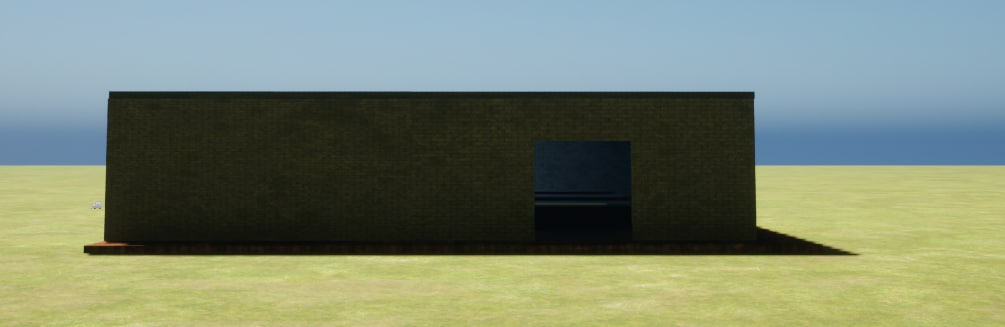
\includegraphics[width=1\textwidth]{img/labof}
	\caption{IHM du laboratoire en vue de face}
	\label{fig:mesh1}
\end{figure}

Il y apparait un locale vue de face et présente l'environnement extérieur du laboratoire oû aurons lieu les réactions.

\subsubsection{Interface du laboratoire intérieur vue du fond}

Cette interface représente une vue interieur du laboratoire vu du fond de la salle.

\begin{figure}[H]
	\centering
	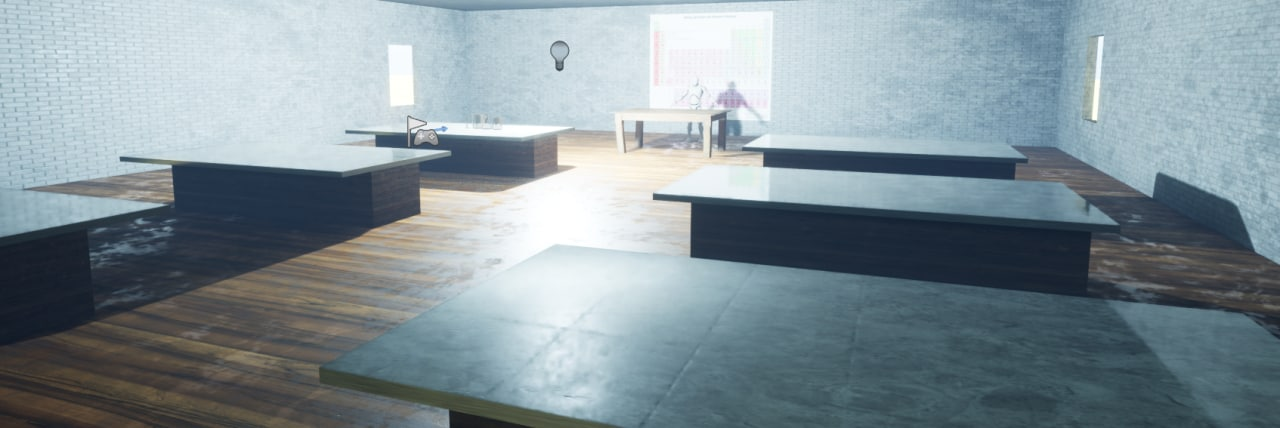
\includegraphics[width=1\textwidth]{img/labo1}
	\caption{IHM du laboratoire intérieur vue du fond}
	\label{fig:mesh1}
\end{figure}

Il y apparait une vue du locale et est présenté l'environnement intérieur du laboratoire avec les tables ou se déroulerons les réactions.

\subsubsection{Interface du laboratoire intérieur vue de l'apprenant}

Cette interface représente le point de vue d'un apprenant qui utilise l'application.

\begin{figure}[H]
	\centering
	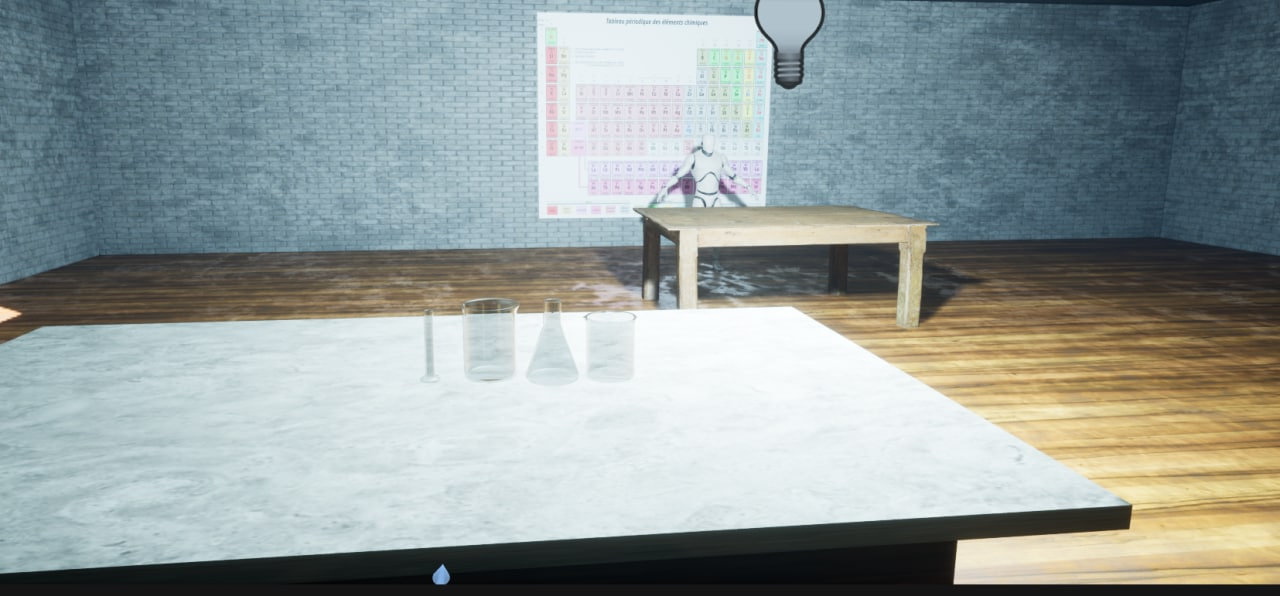
\includegraphics[width=1\textwidth]{img/labo2}
	\caption{IHM du laboratoire intérieur vue de l'apprenant}
	\label{fig:mesh1}
\end{figure}

Il y apparait la table de l'apprenant avec la verrerie des réaction disposé dessus.

\subsubsection{Interface du laboratoire intérieur vue de l'enseignant}

Cette interface représente le point de vue d'un enseignant qui utilise l'application.

\begin{figure}[H]
	\centering
	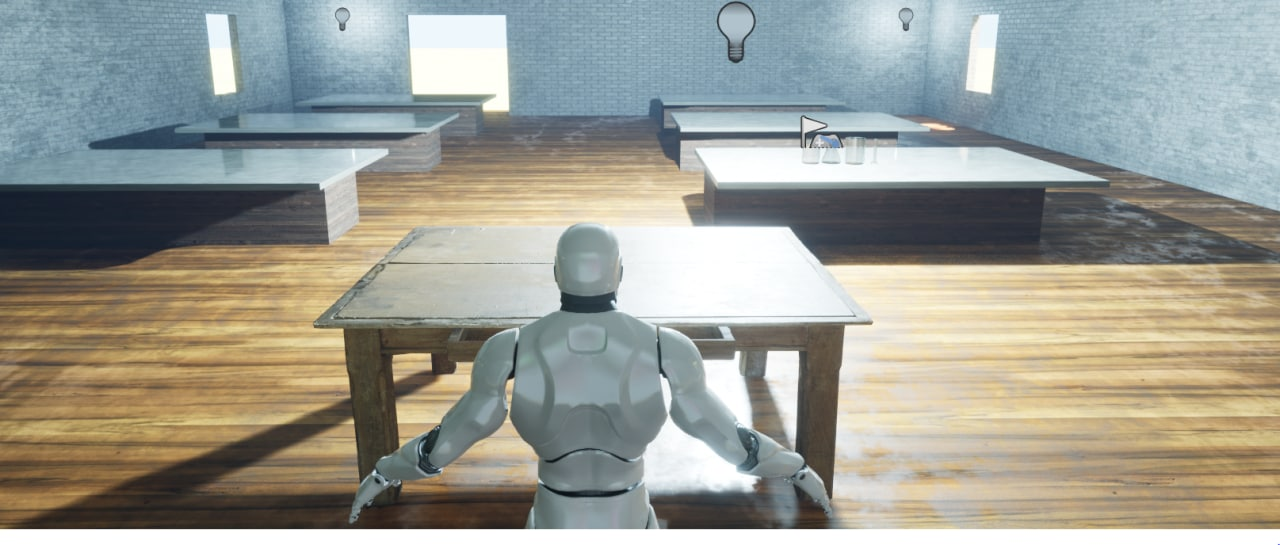
\includegraphics[width=1\textwidth]{img/labo3}
	\caption{IHM du laboratoire intérieur vue de l'enseignant}
	\label{fig:mesh1}
\end{figure}

Il y apparait les tables de réaction des différents apprenants dans le laboratoire virtuel.


\chapter{Implémentation de la solution et résultats}
\textit{Dans ce chapitre, nous ferons un tour d’horizon sur l’ensemble des technologies utilisées
	afin de mettre en œuvre la solution et montrerons comment nous comptons déployer notre
	solution. Enfin nous présenterons quelques résultats obtenus par implémentation.}
\clearpage

\section{Outils et technologies}

De la conception à la réalisation de notre application, nous avons eu à utiliser les outils et technologies suivants :

\begin{itemize}
	\item \textbf{Unreal Engine 5} : qui est un moteur de rendu 3D utilisé dans la création de jeux et la simulation d'environnement 3D utilisant le langage de programmation c++.
	\item \textbf{React \& React Dom} : qui est un Framework javascript très populaire permettant la création d’interfaces utilisateur web simplement et rapidement, il offre une grande documentation et possède une communauté très active.
	\item \textbf{ASP.NET core web api} : est un Framework C\# permettant la création d’api REST développé par Microsoft.
	\item \textbf{PostgreSQL} : C’est un système de gestion de base de données relationnelle et objet. C'est un outil libre disponible selon les termes d'une licence de type BSD. Ce système est concurrent d'autres systèmes de gestion de base de données, qu'ils soient libres, ou propriétaires ;
	\item \textbf{Git \& GitHub} : Git est un logiciel de gestion de versions décentralisé. C'est un logiciel libre créé par Linus Torvalds, auteur du noyau Linux, et distribué selon les termes de la licence publique générale GNU version 2. GitHub est un logiciel libre de forge basé sur git proposant les fonctionnalités de wiki, un système de suivi des bugs, l’intégration continue et la livraison continue ;
	\item \textbf{Rider} : C’est un environnement de développement .NET multiplateforme de chez jetbrains basé sur la plateforme IntelliJ et ReSharper.
	\item \textbf{Webstorm} : C’est un IDE pour les langages Web, développé par l'entreprise JetBrains et basé sur la plateforme IntelliJ IDEA ;
	\item \textbf{Docker} : C’est un IDE pour les langages Web, développé par l'entreprise JetBrains et basé sur la plateforme IntelliJ IDEA ;
	\item \textbf{Jira} : est un système de suivi de bugs, de gestion des incidents et de gestion de projets développé par Atlassian.
	\item \textbf{Visual paradigme} : C’est un outil UML CASE prenant en charge UML 2, SysML et la notation de modélisation de processus métier (BPMN) d’Object Management Group (OMG). Outre la modélisation, il offre des fonctionnalités de génération de rapports et d’ingénierie de code, y compris la génération de code.
	\item \textbf{Gantt Project} : est un logiciel libre de gestion de projet écrit en Java.
\end{itemize}

\section{Résultats}

\subsection{Édition du profile utilisateur}

\subsubsection{Interface d'édition du profile utilisateur}

Il est question de l'interface qui permettra à un utilisateur en occurence un administrateur ou un enseignant de modifier ses information personnelles.

\begin{figure}[H]
	\centering
	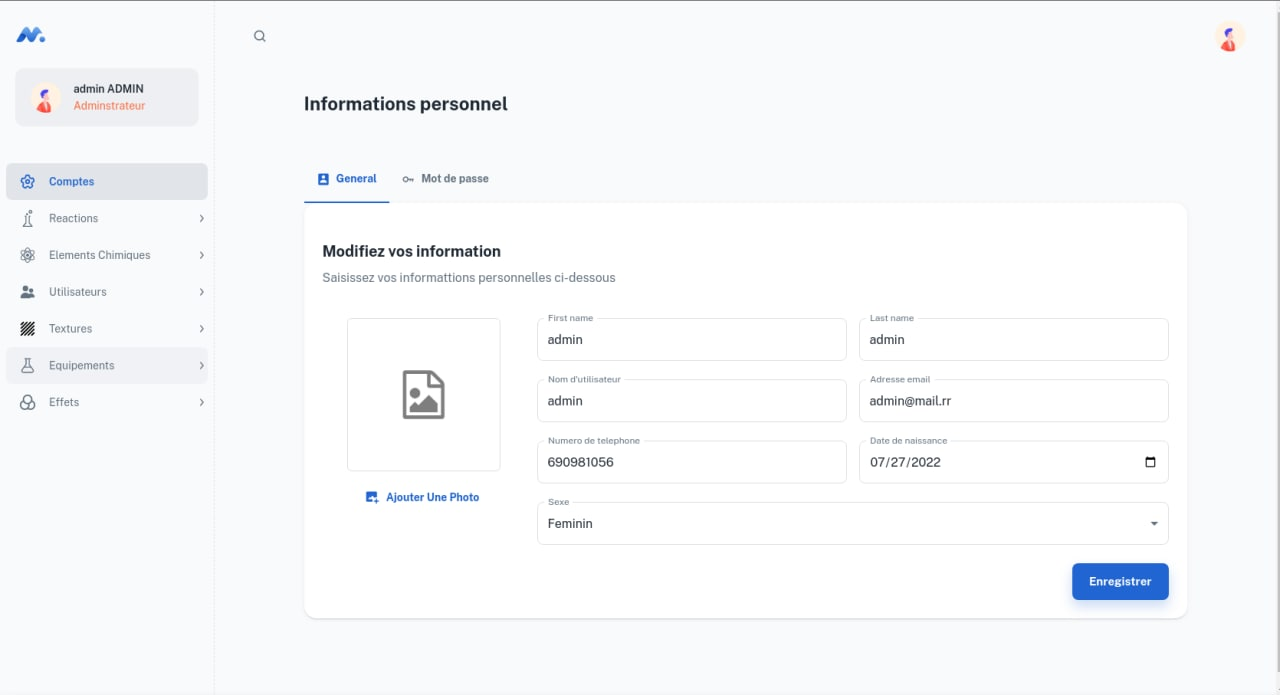
\includegraphics[width=1\textwidth]{img/editpr}
	\caption{IHM formulaire d'édition du profile utilisateur}
	\label{fig:mesh1}
\end{figure}

Il y apparait à gauche les différents menus disponibles de l'application, et à gauche une zone de fomulaire permettant la modification des informations d'un utilisateur.

\subsubsection{Code source backend}

\begin{figure}[H]
	\centering
	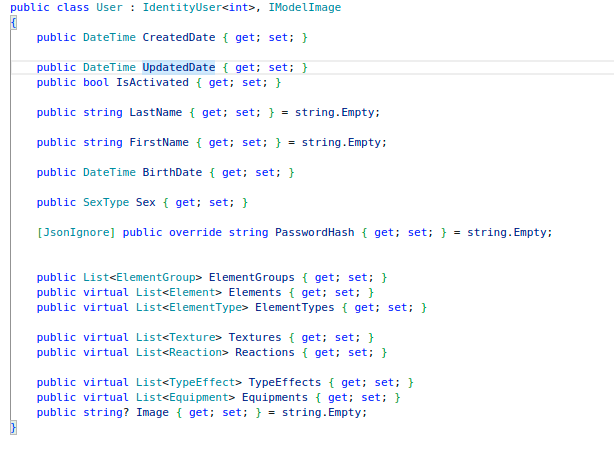
\includegraphics[width=1\textwidth]{img/codeuu}
	\caption{Code backend du model d'utilisateur}
	\label{fig:mesh1}
\end{figure}

Il est question ici de la définition du model d'utilisateur qui sera stocké en base de données.

\begin{figure}[H]
	\centering
	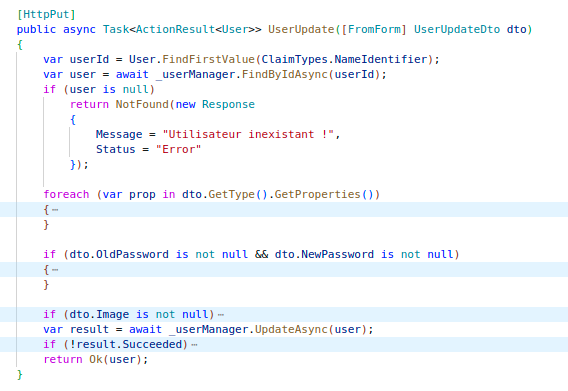
\includegraphics[width=1\textwidth]{img/codeuup}
	\caption{Code backend du cas d'utilisation de l'édition du profile utilisateur}
	\label{fig:mesh1}
\end{figure}

Il est question ici d'une partie du code du controller permettant la gestion des utilisateurs avec la fonctionnalités d'édition des comptes utilisateurs.

\begin{figure}[H]
	\centering
	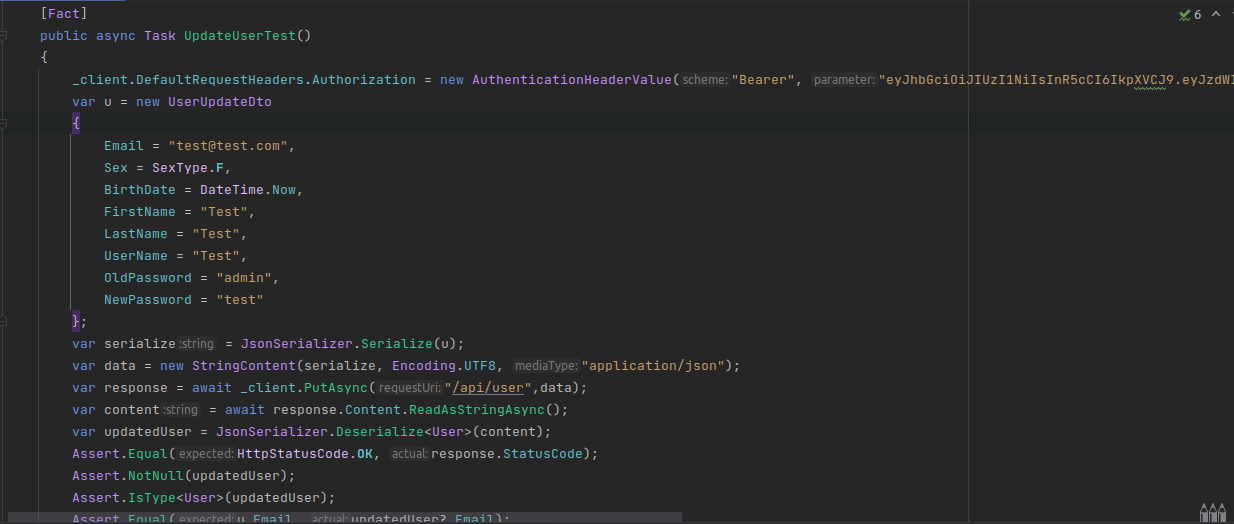
\includegraphics[width=1\textwidth]{img/utupdate}
	\caption{Code backend du test unitaire du cas d'utilisation de l'édition du profile utilisateur}
	\label{fig:mesh1}
\end{figure}

Il est question ici d'une partie du code de test de la fonctionnalités d'édition du profile utilisateur.

\begin{figure}[H]
	\centering
	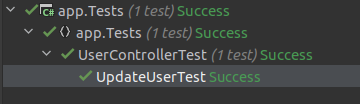
\includegraphics[width=1\textwidth]{img/uutr}
	\caption{Résultat du test unitaire du cas d'utilisation de l'édition du profile utilisateur}
	\label{fig:mesh1}
\end{figure}

Nous avons ici le resultat du test unitaire du cas d'utilisation de l'édition du profile utilisateur, qui s'avère concluent.

\subsubsection{Code source frontend}

\begin{figure}[H]
	\centering
	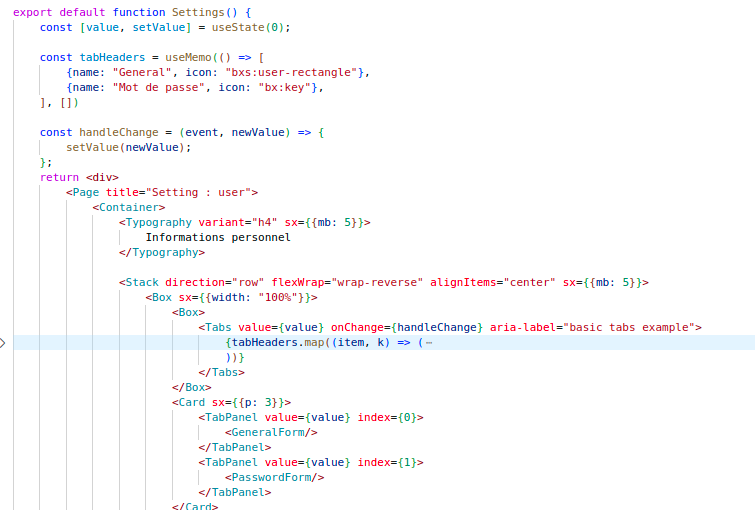
\includegraphics[width=1\textwidth]{img/fuu}
	\caption{Code frontend du cas d'utilisation de l'édition du profile utilisateur}
	\label{fig:mesh1}
\end{figure}

Il est question ici du code React permettant le rendu de la page d'édition du profile utilisateur.

\subsection{Creation des éléments chimiques}

\subsubsection{Interface de creation des éléments chimiques}

\begin{figure}[H]
	\centering
	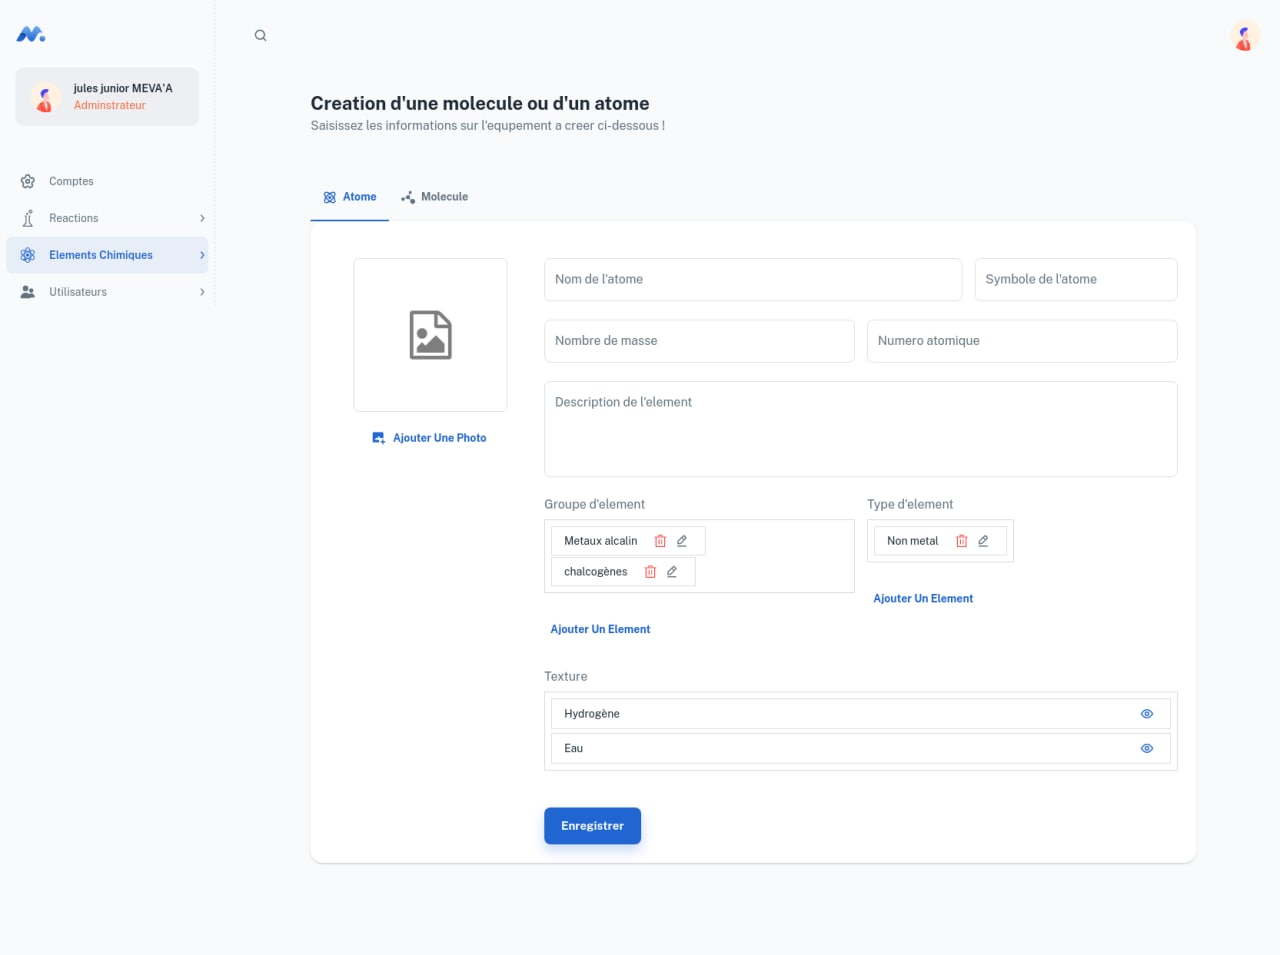
\includegraphics[width=1\textwidth]{img/iec}
	\caption{IHM formulaire de création des éléments chimiques}
	\label{fig:mesh1}
\end{figure}

Ce formulaire permet la création d'un élément chimique (Atome et molécule) et celà en fonction de notre role, seul l'administrateur à le droit de créer des atomes tandis que la création des molécules est autorisée à tous les utilisateurs.

\subsubsection{Code source backend}

\begin{figure}[H]
	\centering
	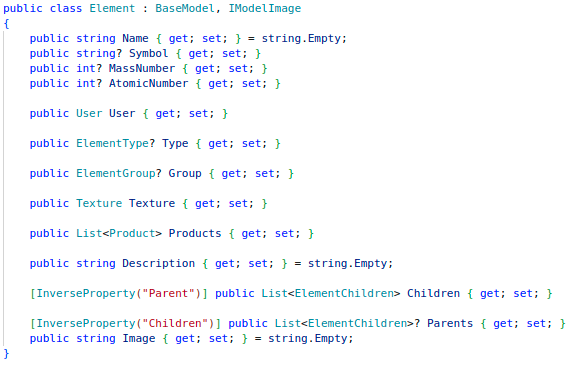
\includegraphics[width=1\textwidth]{img/met}
	\caption{Code backend du model d'élément chimique}
	\label{fig:mesh1}
\end{figure}

Il est question ici de la définition du model d'élément chimique qui sera stocké en base de données.

\begin{figure}[H]
	\centering
	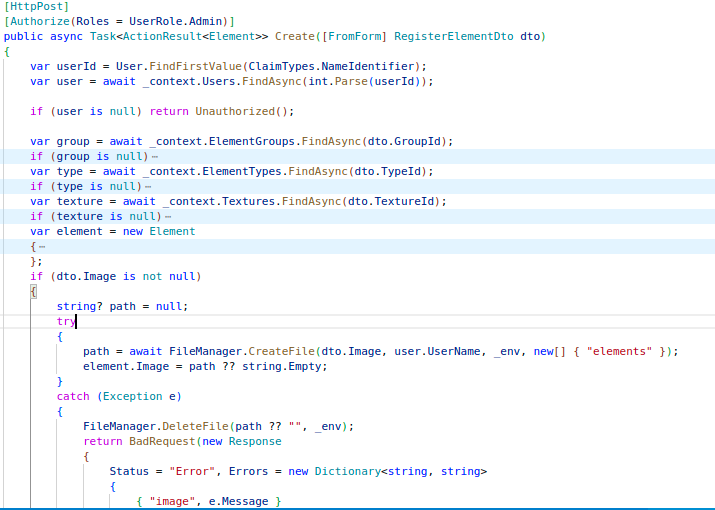
\includegraphics[width=1\textwidth]{img/cep}
	\caption{Code backend du cas d'utilisation de la création d'élément chimique}
	\label{fig:mesh1}
\end{figure}

Il est question ici du code permettant la création d'un élément chimique (atomes).

\begin{figure}[H]
	\centering
	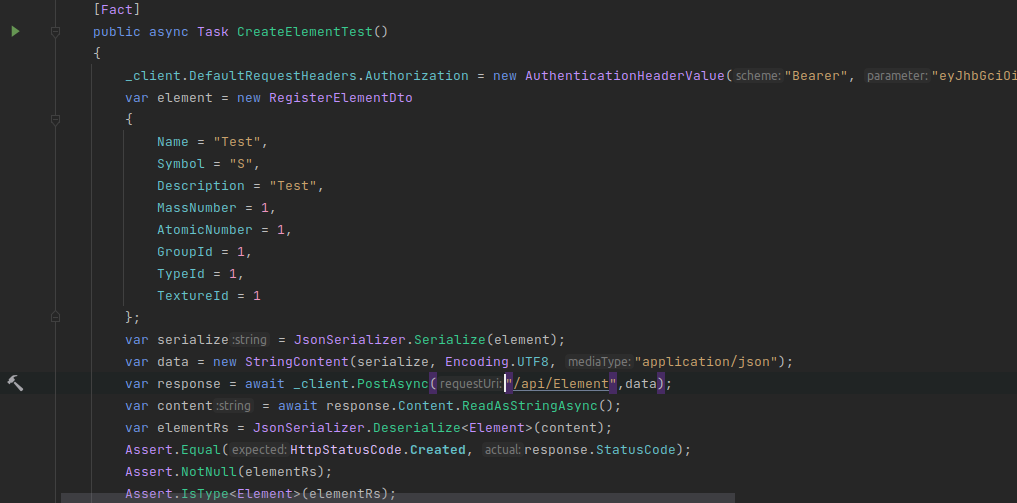
\includegraphics[width=1\textwidth]{img/cet}
	\caption{Code backend du test unitaire du cas d'utilisation de la création d'élément chimique}
	\label{fig:mesh1}
\end{figure}

Il est question ici d'une partie du code de test de la fonctionnalités de création d'élément chimique.

\begin{figure}[H]
	\centering
	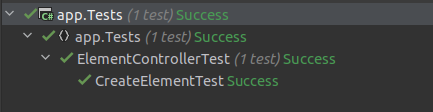
\includegraphics[width=1\textwidth]{img/ute}
	\caption{Résultat du test unitaire du cas d'utilisation de la création d'élément chimique}
	\label{fig:mesh1}
\end{figure}

Nous avons ici le resultat du test unitaire du cas d'utilisation de la création d'élément chimique, qui s'avère concluent.

\subsubsection{Code source frontend}

\begin{figure}[H]
	\centering
	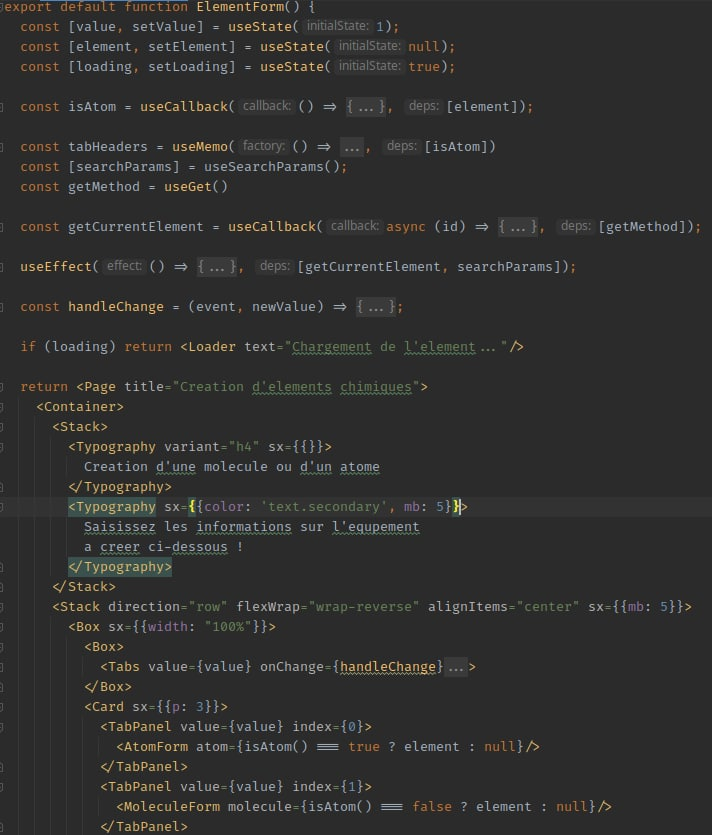
\includegraphics[width=1\textwidth]{img/fec}
	\caption{Code frontend du cas d'utilisation de la création d'élément chimique}
	\label{fig:mesh1}
\end{figure}

Il est question ici du code React permettant le rendu de la page de création d'élément chimique.

\subsection{Listing des éléments chimiques}

\subsubsection{Interface de listing des éléments chimiques}

\begin{figure}[H]
	\centering
	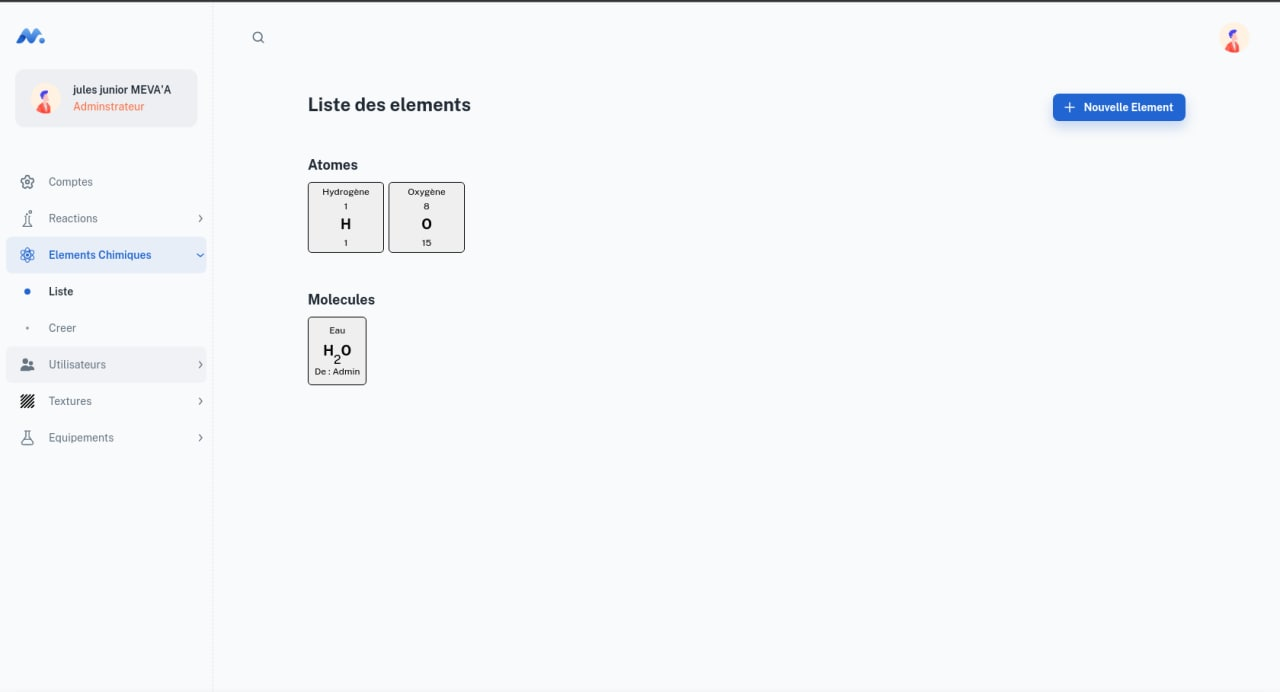
\includegraphics[width=1\textwidth]{img/ietl}
	\caption{IHM du listing des éléments chimiques}
	\label{fig:mesh1}
\end{figure}

Cette interface permet la listing des éléments chimiques (Atome et molécule) enregistrés dans la base de données.

\subsubsection{Code source backend}

\begin{figure}[H]
	\centering
	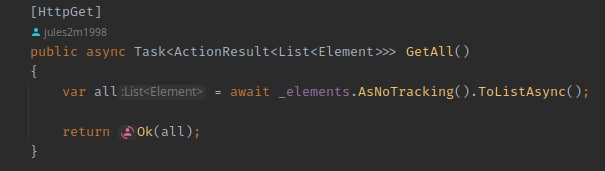
\includegraphics[width=1\textwidth]{img/cetl}
	\caption{Code backend du controller de listing des éléments chimiques}
\end{figure}

Il est question ici du code backend permettant la recupération des élements chimiques en base de données afin de les communiquer à l'interface pour un rendu à l'utilisateur (enseignants ou administrateurs).

\begin{figure}[H]
	\centering
	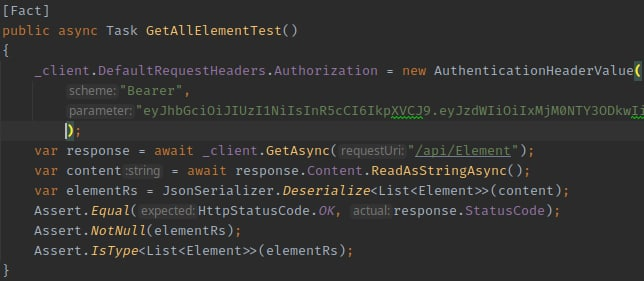
\includegraphics[width=1\textwidth]{img/utetlist2}
	\caption{Code backend du test unitaire du cas d'utilisation de la listing des éléments chimiques}
\end{figure}

Il est question ici du code de test unitaire de la fonctionnalités de listing des éléments chimiques.

\begin{figure}[H]
	\centering
	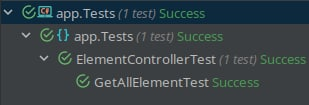
\includegraphics[width=1\textwidth]{img/utetlist}
	\caption{Resultat du test unitaire de la fonctionnalités de listing des éléments chimiques}
\end{figure}

Nous avons ici le resultat du test unitaire de la fonctionnalités de listing des éléments chimiques, qui s'avère concluent.

\subsubsection{Code source frontend}

\begin{figure}[H]
	\centering
	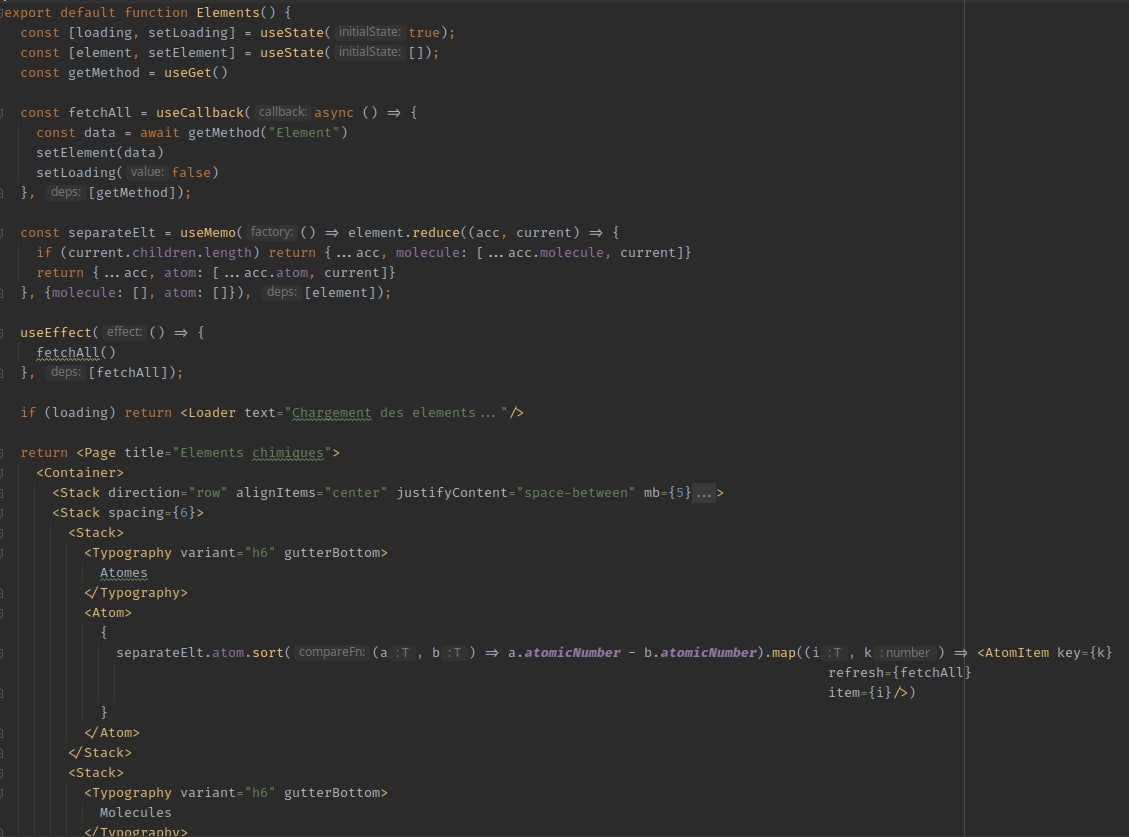
\includegraphics[width=1\textwidth]{img/fetl}
	\caption{Code frontend du cas d'utilisation de la listing des éléments chimiques}
\end{figure}

Il est question ici du code React permettant le rendu de la page de listing des éléments chimiques.

\subsection{Création des réactions chimiques}

\subsubsection{Interface du formulaire de création des réactions chimiques}

\begin{figure}[H]
	\centering
	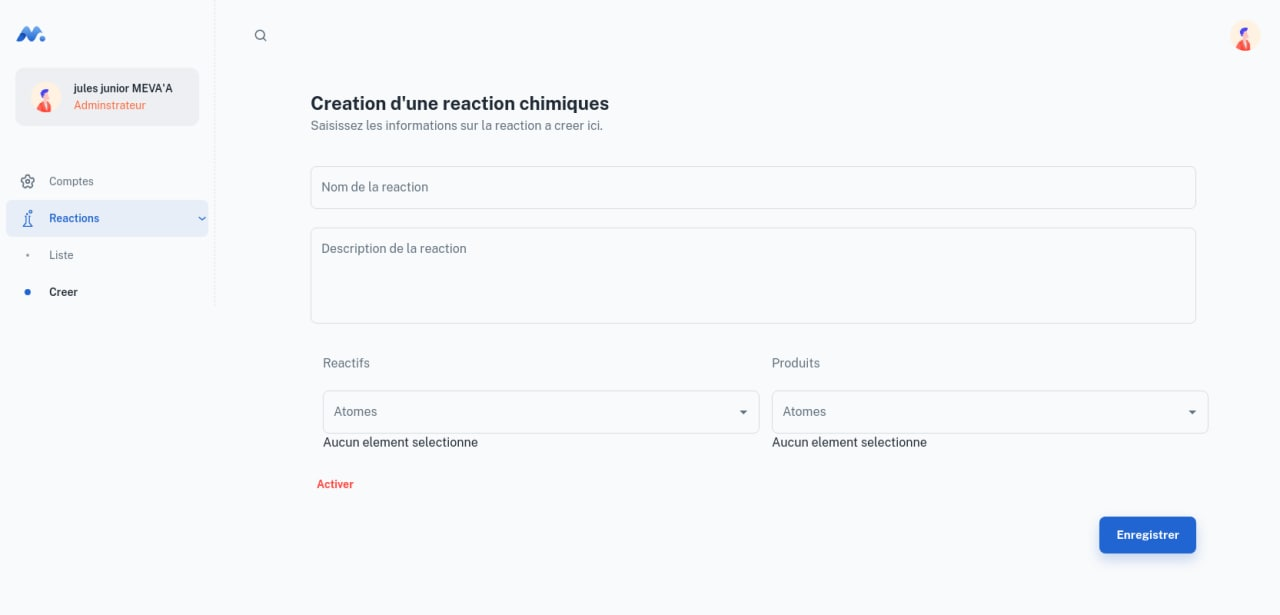
\includegraphics[width=1\textwidth]{img/icrc}
	\caption{IHM formulaire de création des réactions chimiques}
\end{figure}

Ce formulaire permet la création d'une réaction chimique à un utilisateur. Il est question ici de lui donner un nom, un description,
lister les réactifs et les produits de la réaction et de l'activer ou la désactiver.

\subsubsection{Code source backend}

\begin{figure}[H]
	\centering
	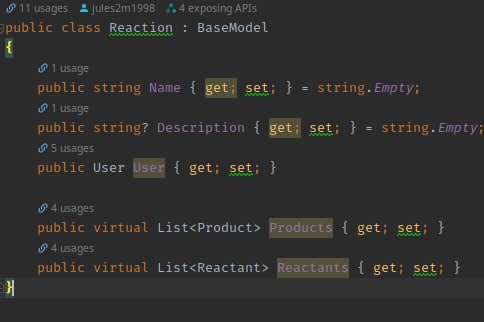
\includegraphics[width=1\textwidth]{img/mre}
	\caption{Code backend du model de réaction}
\end{figure}

Il est question ici de la représentation du modèle d'une réaction chimique qui sera stocké en base de données.

\begin{figure}[H]
	\centering
	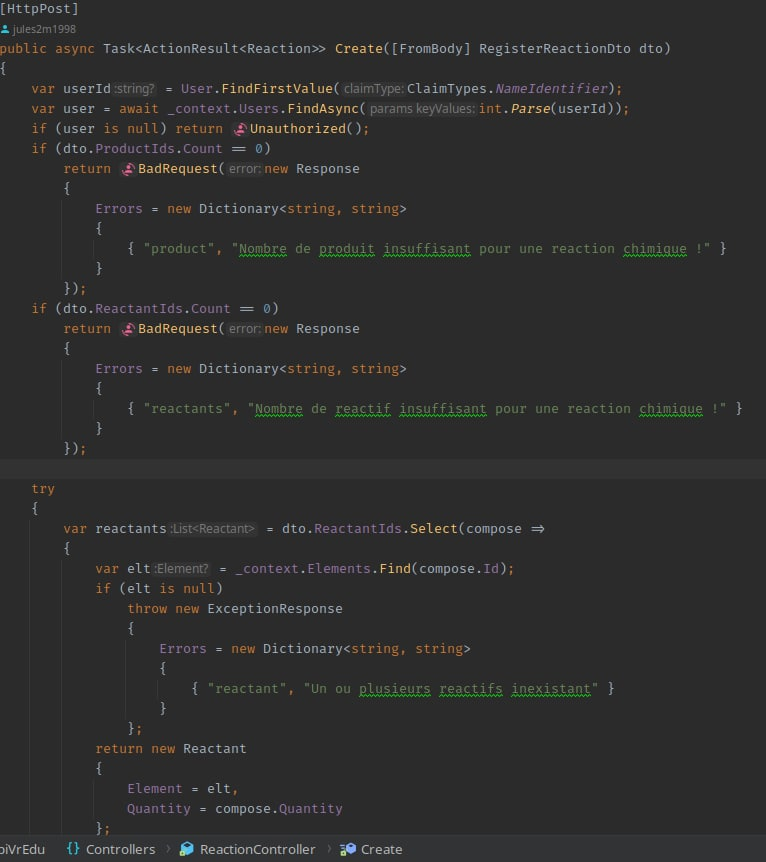
\includegraphics[width=1\textwidth]{img/crec}
	\caption{Code backend du controller de création des réactions chimiques}
\end{figure}

Il est question ici du code permettant la sauvegarde en base de données d'une réaction chimique, cette action n'est possible qu'une fois authentifié.

\begin{figure}[H]
	\centering
	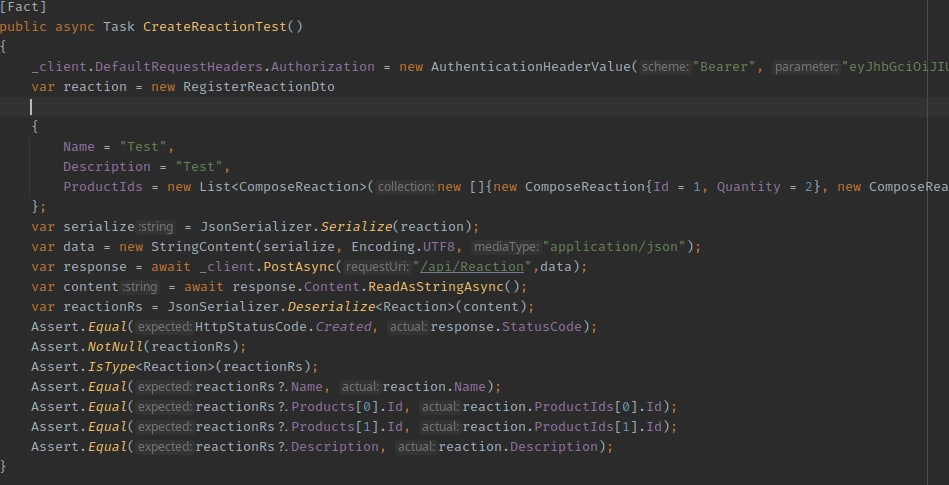
\includegraphics[width=1\textwidth]{img/creac}
	\caption{Code backend du test unitaire du cas d'utilisation de la création d'une réaction chimique}
\end{figure}

Il est question ici d'une partie du code de test de la fonctionnalités de création d'une réaction chimique.

\begin{figure}[H]
	\centering
	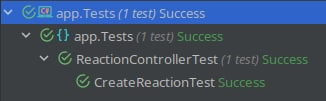
\includegraphics[width=1\textwidth]{img/utcre}
	\caption{Resultat du test unitaire de la fonctionnalités de création d'une réaction chimique}
\end{figure}

Nous avons ici le resultat du test unitaire de la fonctionnalités de création d'une réaction chimique, qui s'avère concluent.

\subsubsection{Code source frontend}

\begin{figure}[H]
	\centering
	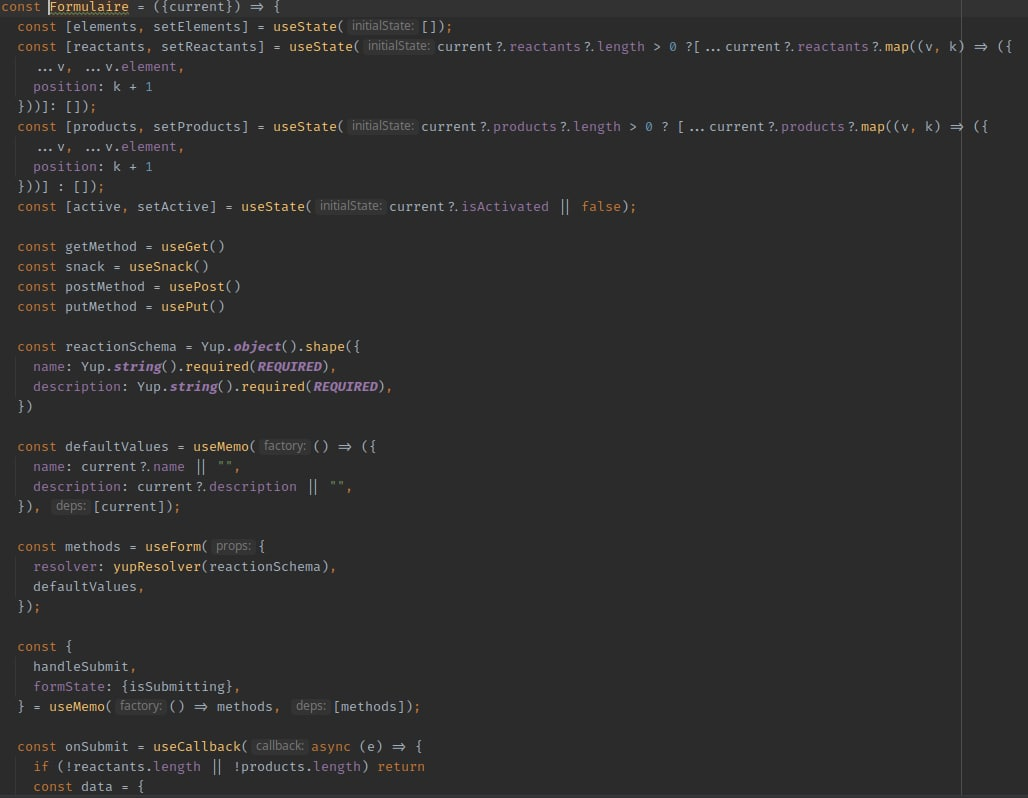
\includegraphics[width=1\textwidth]{img/frec}
	\caption{Code frontend du cas d'utilisation de la création d'une réaction chimique}
\end{figure}

Il est question ici du code React permettant le rendu de la page de création d'une réaction chimique.

\subsection{Listing des réactions chimiques}

\subsubsection{Interface de listing des réactions chimiques}

\begin{figure}[H]
	\centering
	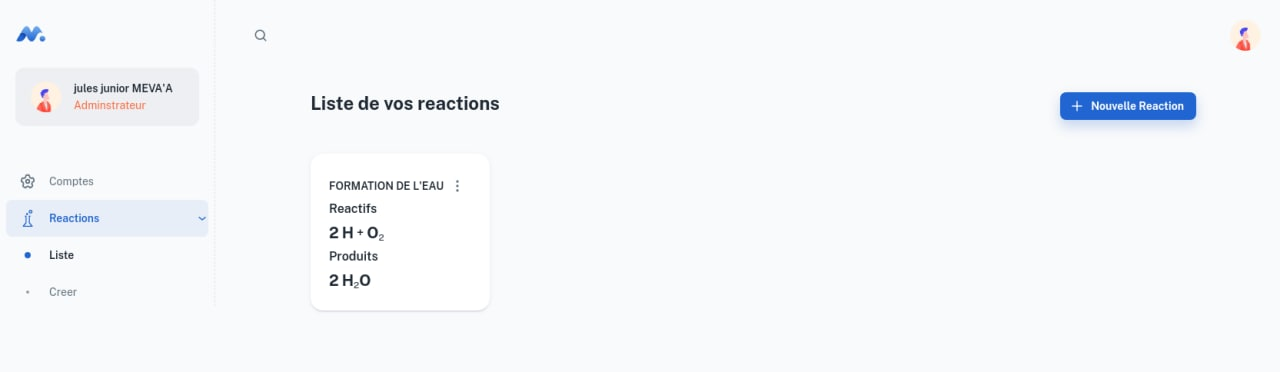
\includegraphics[width=1\textwidth]{img/ilrc}
	\caption{IHM du listing des réactions chimiques}
\end{figure}

Cette interface permet de lister les réactions d'un utilisateur connecté.

\subsubsection{Code source backend}

\begin{figure}[H]
	\centering
	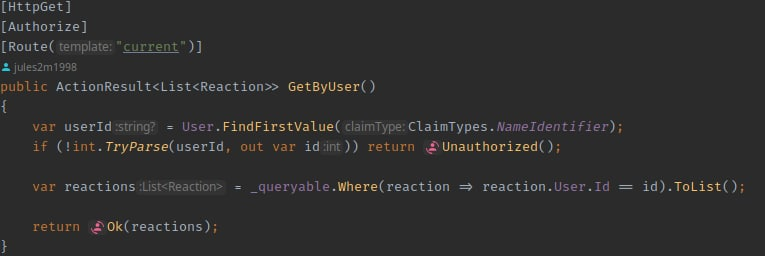
\includegraphics[width=1\textwidth]{img/clrea}
	\caption{Code backend du controller de listing des réactions chimiques}
\end{figure}

Il est question ici du code backend permettant la recupération en base de données des réactions chimiques créé par l'utilisateur connecté afin de les communiquer à l'interface pour un rendu.

\begin{figure}[H]
	\centering
	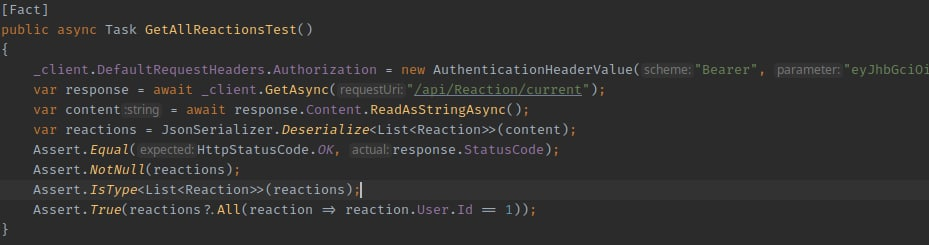
\includegraphics[width=1\textwidth]{img/utreaall}
	\caption{Code backend du test unitaire du cas d'utilisation de la listing des réactions chimiques}
\end{figure}

Il est question ici du code de test unitaire de la fonctionnalités de listing des réactions chimiques.

\begin{figure}[H]
	\centering
	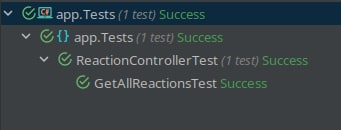
\includegraphics[width=1\textwidth]{img/utrcr}
	\caption{Resultat du test unitaire de la fonctionnalités de listing des réactions chimiques}
\end{figure}

Nous avons ici le resultat du test unitaire de la fonctionnalités de listing des réactions chimiques, qui s'avère concluent.

\subsubsection{Code source frontend}

\begin{figure}[H]
	\centering
	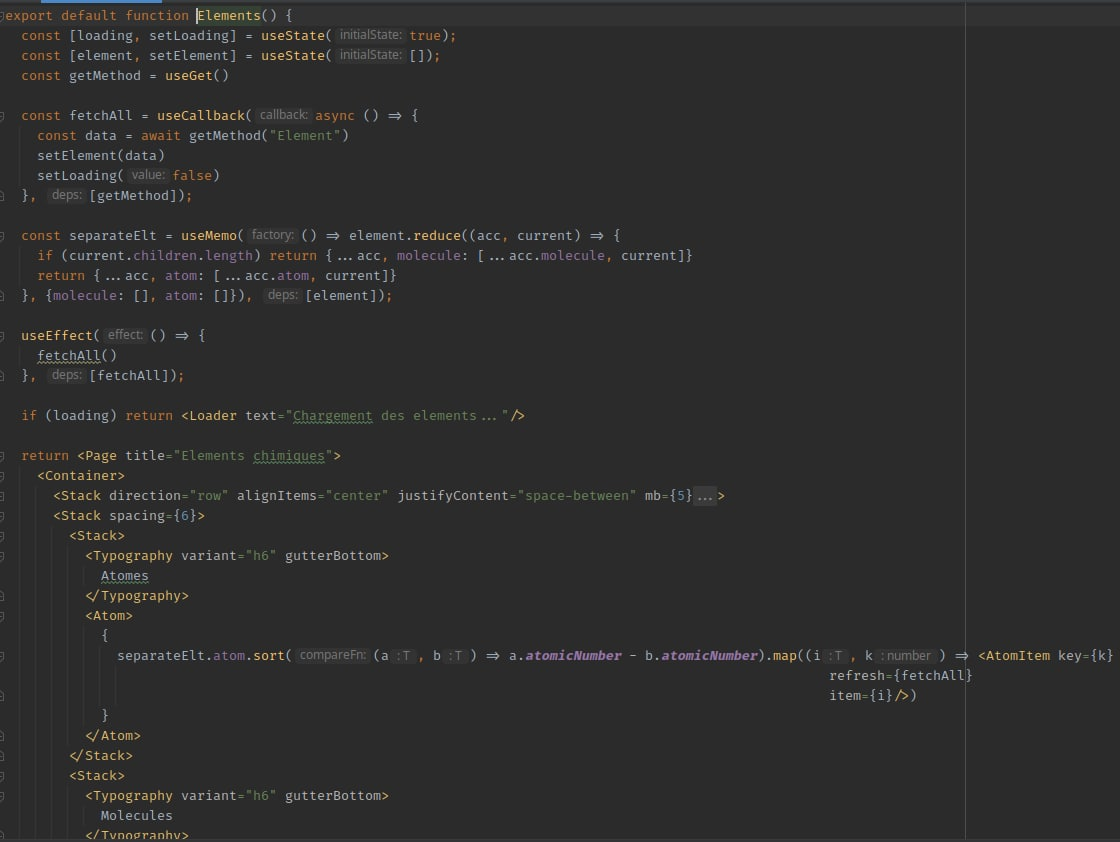
\includegraphics[width=1\textwidth]{img/frl}
	\caption{Code frontend du cas d'utilisation de la listing des réactions chimiques}
\end{figure}

Il est question ici du code React permettant le rendu de la page de listing des réactions chimiques.